\documentclass[12pt,a4wide]{report}
\usepackage{multicol}
\usepackage{amsthm,amssymb,mathrsfs,setspace,pstricks,booktabs,mathtools,amsmath}
%latexsym,footmisc

\usepackage{play}
\usepackage{epsfig}
%\usepackage[grey,times]{quotchap}
\usepackage[nottoc]{tocbibind}
\renewcommand{\chaptermark}[1]{\markboth{#1}{}}
\renewcommand{\sectionmark}[1]{\markright{\thesection\ #1}}
%

\input xy
\xyoption{all}

\setlength{\parskip}{1em plus 0.25em minus 0.25em}

\theoremstyle{plain}
\newtheorem{theorem}{Theorem}[section]
\newtheorem{lemma}[theorem]{Lemma}
\newtheorem{corollary}[theorem]{Corollary}
\newtheorem{proposition}[theorem]{Proposition}

\theoremstyle{definition}
\newtheorem{definition}[theorem]{Definition}
\newtheorem{example}[theorem]{Example}
\newtheorem{notation}[theorem]{Notation}

\theoremstyle{remark}
\newtheorem{remark}[theorem]{Remark}

\renewcommand{\baselinestretch}{1.5}
\newcommand{\reals}{\mathbb{R}}
\newcommand{\jacobian}{\mathcal{J}}
\newcommand{\tallstrut}{\vphantom{\frac{5_A}{4,10^3}}}
\newcommand{\norm}[1]{\left\lVert #1 \right\rVert}

\begin{document}

% --------------- Title page -----------------------
\begin{titlepage}
\enlargethispage{3cm}

\begin{center}

\vspace*{-1cm}

\textbf{\Large A Seminar Report \\on\\ Native Application Development Using Flutter }\\[10pt]

\vspace*{0.5cm}


                         A Seminar Report Submitted \\
                     in Partial Fulfilment of the Requirements  \\
                     for the   \\
                          \vspace{5mm}
                   {\Large \bf Diploma in  } \\
                   in \\
                   {\large \bf Information Technology } \\

                      \vspace{10mm}
                   {\em  by} \\ \vspace{3mm}
             {\large \bf Pratyay Prasad Dhond} \\
{\large \bf (Roll No: 1907011)}\\[.3in]

\vfill

\begin{figure}[h]
  \begin{center}
  
\includegraphics[height=35mm]{Images & Logos/gpn_logo.png}
  \end{center}
\end{figure}
\vspace*{0.1cm}

%{\em\large to }\\%[8pt]
{\bf\large Department of Information Technology} \\%[4pt]
{\bf\large Government Polytechnic, Nagpur}\\%[4pt]
{\bf\large Near Mangalwari Bazar,Sadar, Nagpur 440 001 (M.S.) }\\%[2pt]
{\it\large [A Y 2021-22]}

\end{center}

\end{titlepage}

\clearpage


% --------------- Declaration page -----------------------
\begin{center}
{\Large{\bf{DECLARATION}}}
\end{center}

\noindent

I, \textbf{Pratyay Prasad Dhond (Roll No: 1907011)}, hereby declare that, this report entitled \textbf{``Flutter Internship Report”} submitted to Department of Information Technology, Government Polytechnic Nagpur towards
partial requirement of \textbf{ Diploma} in \textbf{Information Technology.} 
\par Industrial Training work carried out by me under the supervision of \textbf{Prof. S J Pukale }Sir, and \textbf{Soumitra Mahajan} sir, Whenever an external information or statement or result is used then, that have been duly acknowledged and cited.

\vspace{4cm}

\noindent Place:-Government Polytechnic, Nagpur \hfill \textbf{Pratyay Prasad Dhond}

\noindent Date:-[\today]

\clearpage


% --------------- Certificate page -----------------------
\begin{center}
{\Large{\bf{CERTIFICATE}}}
\end{center}

\noindent

This is to certify that the Seminar Report entitled \textbf{Native Application Development Using Flutter} Submitted by \textbf{Pratyay Prasad Dhond (Roll No: 1907011)}, is a bonafide work carried out under the supervision of \textbf{Dr. A. R. Mahajan} and it is submitted towards the partial fulfilment of the requirement Government Polytechnic,Nagpur for the award of the Diploma in Information Technology.
\vskip 0.6in
\begin{center}
\begin{multicols}{2}
{ \bf Dr. A. R. Mahajan}\\Guide-Lecturer,\\Department of Information Technology\\.\\
{\bf Dr.A R Mahajan}\\Head of the Department,\\Department of Information Technology\\

\end{multicols}
\end{center}
\vskip 0.4in
\begin{center}
\begin{multicols}{2}

.\\{\bf Seal/Stamp of the College}\\
{\bf \large Dr. M. B. Daigavane}\\{Principal}

\end{multicols}
\end{center}
\vspace{2cm}

\noindent Place:-Government Polytechnic, Nagpur \hfill 

\noindent Date:-[\today]

\clearpage


% --------------- Abstract page -----------------------
\begin{center}
{\Large{\bf{ABSTRACT}}}
\end{center}

Flutter is a cross-platform User Interface development framework that is used
to develop cross platform applications using a single code base. Flutter can be
used to build beautiful, natively compiled application for various platforms such
as Android, iOS, Windows, Mac, Linux, Web, etc. using a single codebase.

The key features of the Flutter Framework are Fast Development using the
Hot Reload, Expressive and Flexible User Interface(UI) and the Native Performance.

Fast Development : Flutter’s hot reload helps you quickly and easily experiment, build UIs, add features, and fix bugs faster. Experience sub-second reload
times without losing state on emulators, simulators, and hardware.

Expressive, beautiful UIs: Flutter comes with easy to build, highly customizable UI widgets which can be used for easy development. Flutter also supports custom widget building using other widgets.
Native Performance : Flutter’s widgets incorporate all critical platform
differences such as scrolling, navigation, icons and fonts to provide full native
performance on both iOS and Android.
\clearpage
\tableofcontents
\clearpage
\listoffigures
\listoftables

\newpage

\pagenumbering{arabic}
\setcounter{page}{1}

% =========== Main chapters starts here. Type in seperate files and include the filename here. ==
% ============================

\chapter{Introduction}

If you ask ten different mobile developers how they develop their mobile applications for Android or iOS devices, you’ll probably get 10 different answers. This use of different languages for different Operating systems creates the need of employment of development teams for each operating system like Android, iOS, Windows, Mac, Linux, as well as web-apps,etc. This severely affects the cost of the project to build. As with every project to be built there is a need for different meetings, development phases, testing phases, designing phases, different codebases and ultimately these softwares are hard to manage as a change in the software will need the change to be reflected in each and every code base individually by the different teams.

To avoid this reason there was a need for cross platform development from
the old-fashioned porting of apps. For solving this problem, Google developed the
flutter framework to make cross platform development easier, with the view of
-’One codebase, multiple platforms!’. 



\section{History}

The principal adaptation of Flutter was known by the codename "Sky" and ran on the Android operating framework. It was revealed at the 2015 Dart engineer summit with the expressed expectation of having the option to deliver reliably at 120 frames per second. During the feature of Google Developer Days in Shanghai in September 2018, Google declared Flutter Release Preview 2, which is the last large delivery before Flutter 1.0. On December fourth of that year, Flutter 1.0 was delivered at the Flutter Live occasion, meaning the principal "stable" variant of the Framework. On December 11, 2019, Flutter 1.12 was delivered at the Flutter Interactive event.

On May 6, 2020, the Dart programming advancement unit (SDK) in variant 2.8 and the Flutter in form 1.17.0 were delivered, where backing was added to the Metal API, further developing execution on iOS gadgets (around half), new Material gadgets, and new organization following.

On March 3, 2021, Google delivered Flutter 2 during an internet based Flutter Engage occasion. This significant update brought official help for online applications with new Canvas Kit renderer and web explicit gadgets, early-access desktop application support for Windows, macOS, and Linux and further developed Add-to-App APIs. This delivery included sound invalid wellbeing, which caused many breaking changes and issues with numerous outer bundles, yet the Flutter group included directions to alleviate these progressions also.

On September eighth, 2021, the Dart SDK in variant 2.14 and Flutter adaptation 2.5 were delivered by Google. The update carried upgrades to the Android Full-Screen mode and the most recent variant of Google's Material Design called Material You. Dart got two new updates, the most up to date build up conditions have been normalized and preset as the default conditions too Dart for Apple Silicon is presently steady.


\chapter{Introduction to Dart}
Dart is a programming language designed mainly for client development, such as for the web and mobile apps. Developed by Google, it is gaining popularity quite fast and it can also be used to build server and desktop applications.\\
Dart is an Object-oriented, class based, garbage collected language with C like syntax.\\
Dart can either compile to either native code or to JavaScript\\
It supports interfaces, mixins, abstract classes, reified generics, and type inference.\\

\begin{figure}[h]
  \begin{center}
  
\includegraphics[height=55mm]{Images & Logos/CH02_dart.png}\\
  \end{center}
  \caption{Dart Language}
\end{figure}  

\section{History}
\begin{itemize}
  \item Unveiled at GOTO conference in Aarhus, Denmark, on October 10-12 2012.
  \item The dart project was founded by Lars Bak and Kasper Lund.
  \item Dart 1.0 was released on November 14,2013.
  \item Dart 1.9 released in 2015 to focus on compiling Dart to JavaScript.
  \item Dart 2.0 released in August 2018
  \item Dart 2.6 introduced new extension, dart2native
\end{itemize}



\chapter{Widgets}

Everything in Flutter is a Widget. This incorporates UI components, like ListView,
TextBox, and Image, just as different parts of the system, including format, activity, motion
acknowledgment, and subjects, to give some examples.\\
Widgets are fundamental for an application's view and interface. They should have a characteristic look and
feel paying little heed to screen size. They likewise should be quick, extensible, and adjustable. Flutter takes the
Everything is a Widget approach. It has a rich arrangement of Widgets and broad abilities for making
complex custom Widgets. In Flutter, Widgets aren't just utilized for views. They're additionally utilized for whole
screens and in any event, for the actual application.\\
As Flutter's documentation puts it, every Widget is an unchanging presentation of part of the
UI. Different structures separate perspectives, view regulators, designs, and different properties.
Flutter, then again, has a predictable, consistent, brought together item model: the Widget.
A Widget can characterize an underlying component (like a button or menu); a complex component (like a textual style
or on the other hand color scheme); a part of the format (like padding, etc.
Widgets structure a chain of command dependent on their piece. Every Widget settles within and acquires
properties from its parent. There's no different application object. All things considered, the root Widget serves this
job.\\
Flutter has a full arrangement of Widgets in Google's Material Design and in Apple's style with the
Cupertino pack. Widget delivering happens straightforwardly in the Skia engine without utilizing Original
Equipment Manufacturer Widgets. So we get a smoother UI experience contrasted and other cross
platform structures.\\
\\
Widgets in Flutter are divided into two sub categories:\\
1) StateLess Widgets\\
2) StateFul Widgets\\

\section{StateLess Widgets}

A stateless Widget is a Widget that portrays part of the UI by building a network 
of different Widgets that portray the UI all the more solidly. The building process proceeds
recursively until the description of the UI is completely concrete.\\
\begin{figure}[h]
  \begin{center}
  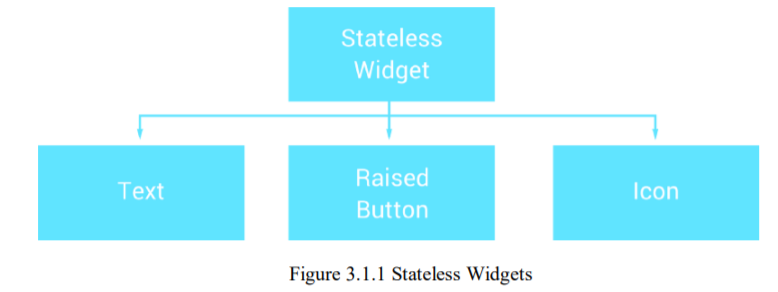
\includegraphics[height=55mm]{Images & Logos/CH_03_STATELESS.png}\\
  \end{center}
  \caption{Stateless Widget}
\end{figure}  

Stateless Widget are valuable when the piece of the UI you are portraying doesn't rely upon something besides the arrangement data in the actual article and the BuildContext in which the Widget is expanded. For compositions that can change dynamically, for example due to having an inside clock-driven state, or relying upon some system state, think about utilizing StatefulWidget.\\

\section{StateFul Widget}
A stateful widget is a widget that describes part of the user interface by building a constellation of other widgets that describe the user interface more concretely. The building process continues recursively until the description of the user interface is fully concrete (e.g., consists entirely of RenderObjectWidgets, which describe concrete RenderObjects).\\

\begin{figure}[h]
  \begin{center}
 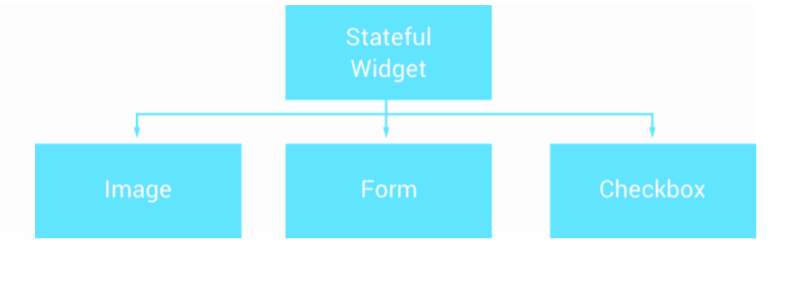
\includegraphics[height=55mm]{Images & Logos/CH_03_STATEFUL.png}
  \end{center}
  \caption{Stateful Widget}
\end{figure}  
Stateful widgets are useful when the part of the user interface you are describing can change dynamically, e.g. due to having an internal clock-driven state, or depending on some system state. For compositions that depend only on the configuration information in the object itself and the BuildContext in which the widget is inflated, consider using StatelessWidget.\\


\chapter{Comparision to other development platforms}




\section{Apple and Android Development}
Native applications offer the least trouble in adopting new features. These Native Applications tend to have user
experiences more in tune with the given platform since the applications are built specifically for the platforms, using the controls from
the platform vendors themselves (Apple or Google) and often they follow design guidelines set out by
these vendors.\\
One big advantage of the native applications is that they can adopt brand new technologies, make changes, and access the APIs for the platform directly with the help of lots of documentation available for the Native application Development framework. Apple
and Google create features available in beta immediately if desired, without having to wait for any third-party
integration. The main disadvantage to building native applications is the lack of code reuse, as the code is specific to the platform, that is it cannot be used across
platforms, which can make development expensive if targeting iOS and Android.

\section{React Native}
React Native allows the software developers to build native applications using JavaScript. The actual controls the
application uses are native platform controls, so the end user gets the feel of a native app. For apps
that require customization beyond what React Native’s abstraction provides, native development could
still be needed.\\ In cases where the amount of customization required is substantial, the benefit of
working within React Native’s abstraction layer lessens to the point where in some cases developing
the app natively would be more beneficial

\chapter{Widgets}

Everything in Flutter is a Widget. This incorporates UI components, like ListView,
TextBox, and Image, just as different parts of the system, including format, activity, motion acknowledgment, and subjects, to give some examples.\\
Widgets are fundamental for an application's view and interface. They should have a characteristic look and
feel paying little heed to screen size. They likewise should be quick, extensible, and adjustable. Flutter takes the
Everything is a Widget approach. It has a rich arrangement of Widgets and broad abilities for making
complex custom Widgets. In Flutter, Widgets aren't just utilized for views. They're additionally utilized for whole
screens and in any event, for the actual application.\\
As Flutter's documentation puts it, every Widget is an unchanging presentation of part of the
UI. Different structures separate perspectives, view regulators, designs, and different properties.
Flutter, then again, has a predictable, consistent, brought together item model: the Widget.
A Widget can characterize an underlying component (like a button or menu); a complex component (like a textual style
or on the other hand color scheme); a part of the format (like padding, etc.
Widgets structure a chain of command dependent on their piece. Every Widget settles within and acquires
properties from its parent. There's no different application object. All things considered, the root Widget serves this
job.\\
Flutter has a full arrangement of Widgets in Google's Material Design and in Apple's style with the
Cupertino pack. Widget delivering happens straightforwardly in the Skia engine without utilizing Original
Equipment Manufacturer Widgets. So we get a smoother UI experience contrasted and other cross
platform structures.\\
\\
Widgets in Flutter are divided into two sub categories:\\
1) StateLess Widgets\\
2) StateFul Widgets\\

\section{StateLess Widgets}

A stateless Widget is a Widget that portrays part of the UI by building a network 
of different Widgets that portray the UI all the more solidly. The building process proceeds
recursively until the description of the UI is completely concrete.\\
\begin{figure}[h]
  \begin{center}
  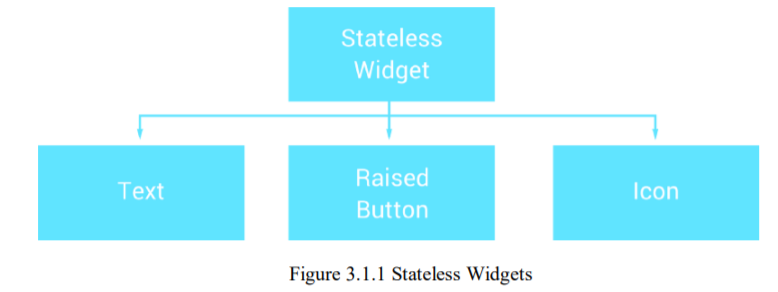
\includegraphics[height=55mm]{Images & Logos/CH_03_STATELESS.png}\\
  \end{center}
  \caption{Stateless Widget}
\end{figure}  

Stateless Widget are valuable when the piece of the UI you are portraying doesn't rely upon something besides the arrangement data in the actual article and the BuildContext in which the Widget is expanded. For compositions that can change dynamically, for example due to having an inside clock-driven state, or relying upon some system state, think about utilizing StatefulWidget.\\

\section{StateFul Widget}
A stateful widget is a widget that describes part of the user interface by building a constellation of other widgets that describe the user interface more concretely. The building process continues recursively until the description of the user interface is fully concrete (e.g., consists entirely of RenderObjectWidgets, which describe concrete RenderObjects).\\

\begin{figure}[h]
  \begin{center}
 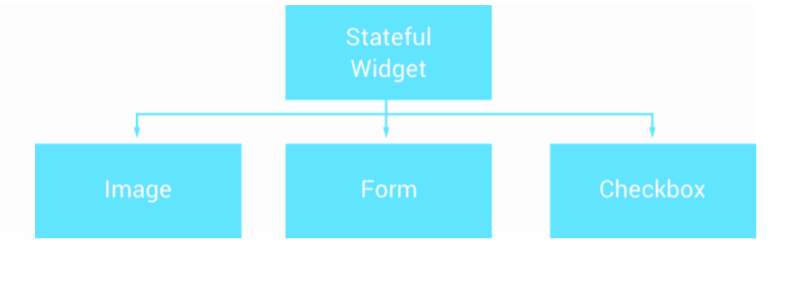
\includegraphics[height=55mm]{Images & Logos/CH_03_STATEFUL.png}
  \end{center}
  \caption{Stateful Widget}
\end{figure}  
Stateful widgets are useful when the part of the user interface you are describing can change dynamically, e.g. due to having an internal clock-driven state, or depending on some system state. For compositions that depend only on the configuration information in the object itself and the BuildContext in which the widget is inflated, consider using StatelessWidget.\\


\chapter{Widget Tree}

\section{Summary}
Developers utilise the widget tree to design user interfaces; they place widgets within each other to create basic and complicated layouts. Because almost everything in the Flutter framework is a widget, the code might get difficult to read when they start layering them. Developers can divide widgets into their own widget class, resulting in a shorter widget tree, which improves code readability and administration. Developers may take advantage of Flutter's subtree rebuilding, which enhances efficiency, by refactoring using a widget class. The widget is initialised to a final variable when you refactor with a constant. The chapter delves into refactoring with a method rather than a constant in depth. By invoking the method name, refactoring with a method returns the widget.\\

\begin{figure}[h]
  \begin{center}
  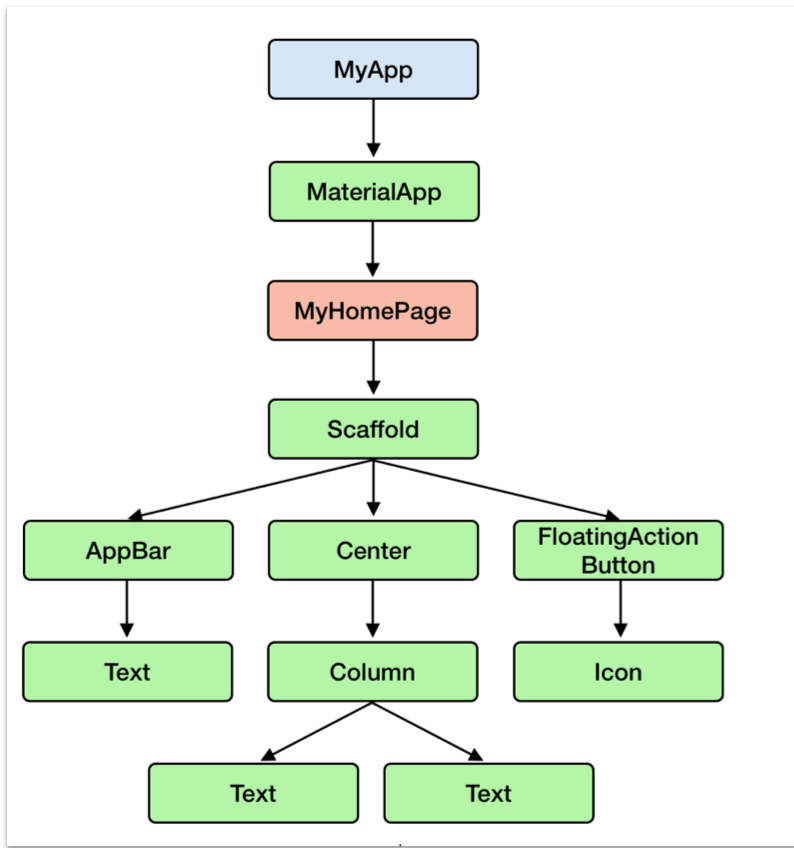
\includegraphics[height=120mm]{Images & Logos/CH_04_Widget_Tree.png}\\
  \end{center}
  \caption{Stateless Widget}
\end{figure}  
	


	\chapter{Flutter Provider Widget}




\section{What is Flutter Provider?}
The provider package is an easy to use package which is basically a wrapper around the InheritedWidgets that makes it easier to use and manage. It provides a state management technique that is used for managing a piece of data around the app.\\


\section{basic classes that are provided with flutter provider}
The basic classes available in the provider package are –\\
ChangeNotifierProvider<T extends ChangeNotifier> It listens to a ChangeNotifier extended by the model class, exposes it to its children and descendants, and rebuilds depends whenever notifyListeners is called.\\
Consumer - It obtains the provider from its ancestors and passes the value obtained to the builder.\\
FutureProvider - This class listens for a Future and then passes its values to its children and descendants.\\
InheritedProvider - The InheritedProvider provides a general implementation of the InheritedWidget.\\
MultiProvider A provider that is used to provide more than one class at the same time.\\
Provider -  It is the basic provider.\\
ProxyProvider - This provider depends on other providers for value. The value can be used by create or update.\\


\chapter{Project}
At the end of the internship, we were assigned a task to develop an application using Flutter. I made a to-do List application, with the following features:\\
\begin{itemize}
\item Login and Signup with Firestore authentication as backend
\item Two user friendly themes (Light theme and dark theme)
\item Minimalistic Design
\item Data synchronisation on Firestore firebase cloud
\end{itemize}
\hfill
\newpage

\subsection{Login and Signup with Firestore Authentication}

\begin{figure}
  \begin{center}
  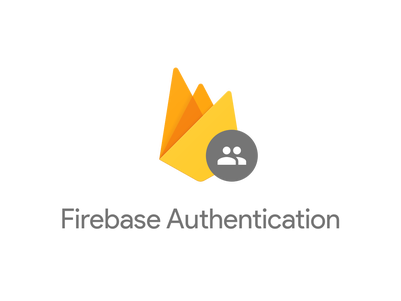
\includegraphics[height=80mm]{Images & Logos/CH_08_FirebaseAuth.png}
  \end{center}
  \caption{Firebase Authentication Logo}
\end{figure}

In the present era, user authentication is one of the most important requirements for Android apps. It is essential to authenticate users, and it is much harder if we have to write all this code on our own. This is done very easily with the help of Firebase.
\begin{itemize}
\item Being able to authenticate our users securely, it offers a customized experience to them based on their interests and preferences.
\item We can ensure that they have no problems accessing their private data while using our app from multiple devices.
\item Firebase Authentication provides all the server-side stuff for authenticating the user. Firebase Authentication becomes easy with SDK. It makes API easy to use.
\item Firebase Authentication also provides some user interface libraries which enable screens for us when we are logging it.
\item Firebase authentication supports authentication using a password, phone numbers, popular identity provider like Google, Facebook, and Twitter, etc.
\item We can sign in users to our app by using the FirebaseUI.
\item It handles the UI flows for signing in user with an email address and password, phone numbers, and popular providers, including Google sign-In and Facebook Login
\item It can also handle cases like account recovery.
\item It is not required to design a UI since it is already provided for us. It means we don't have to write the activities.
\item We can also sign-in users using the Firebase Authentication SDK to integrate one or several sign-in methods into our app manually.

\end{itemize}
\newpage
\section{Two user friendly themes}
In the To-Do List app i created,  i had two themes i.e. dark mode and light mode for the users to have good user experience.

\subsection{Light Mode}
\begin{itemize}
\item White background
\item Grey Buttons (HexCode : \#EAEAEA)
\item Black icons
\item Green Update and Complete task button
\end{itemize}
%\begin{figure}[h]
%  \begin{center}
%   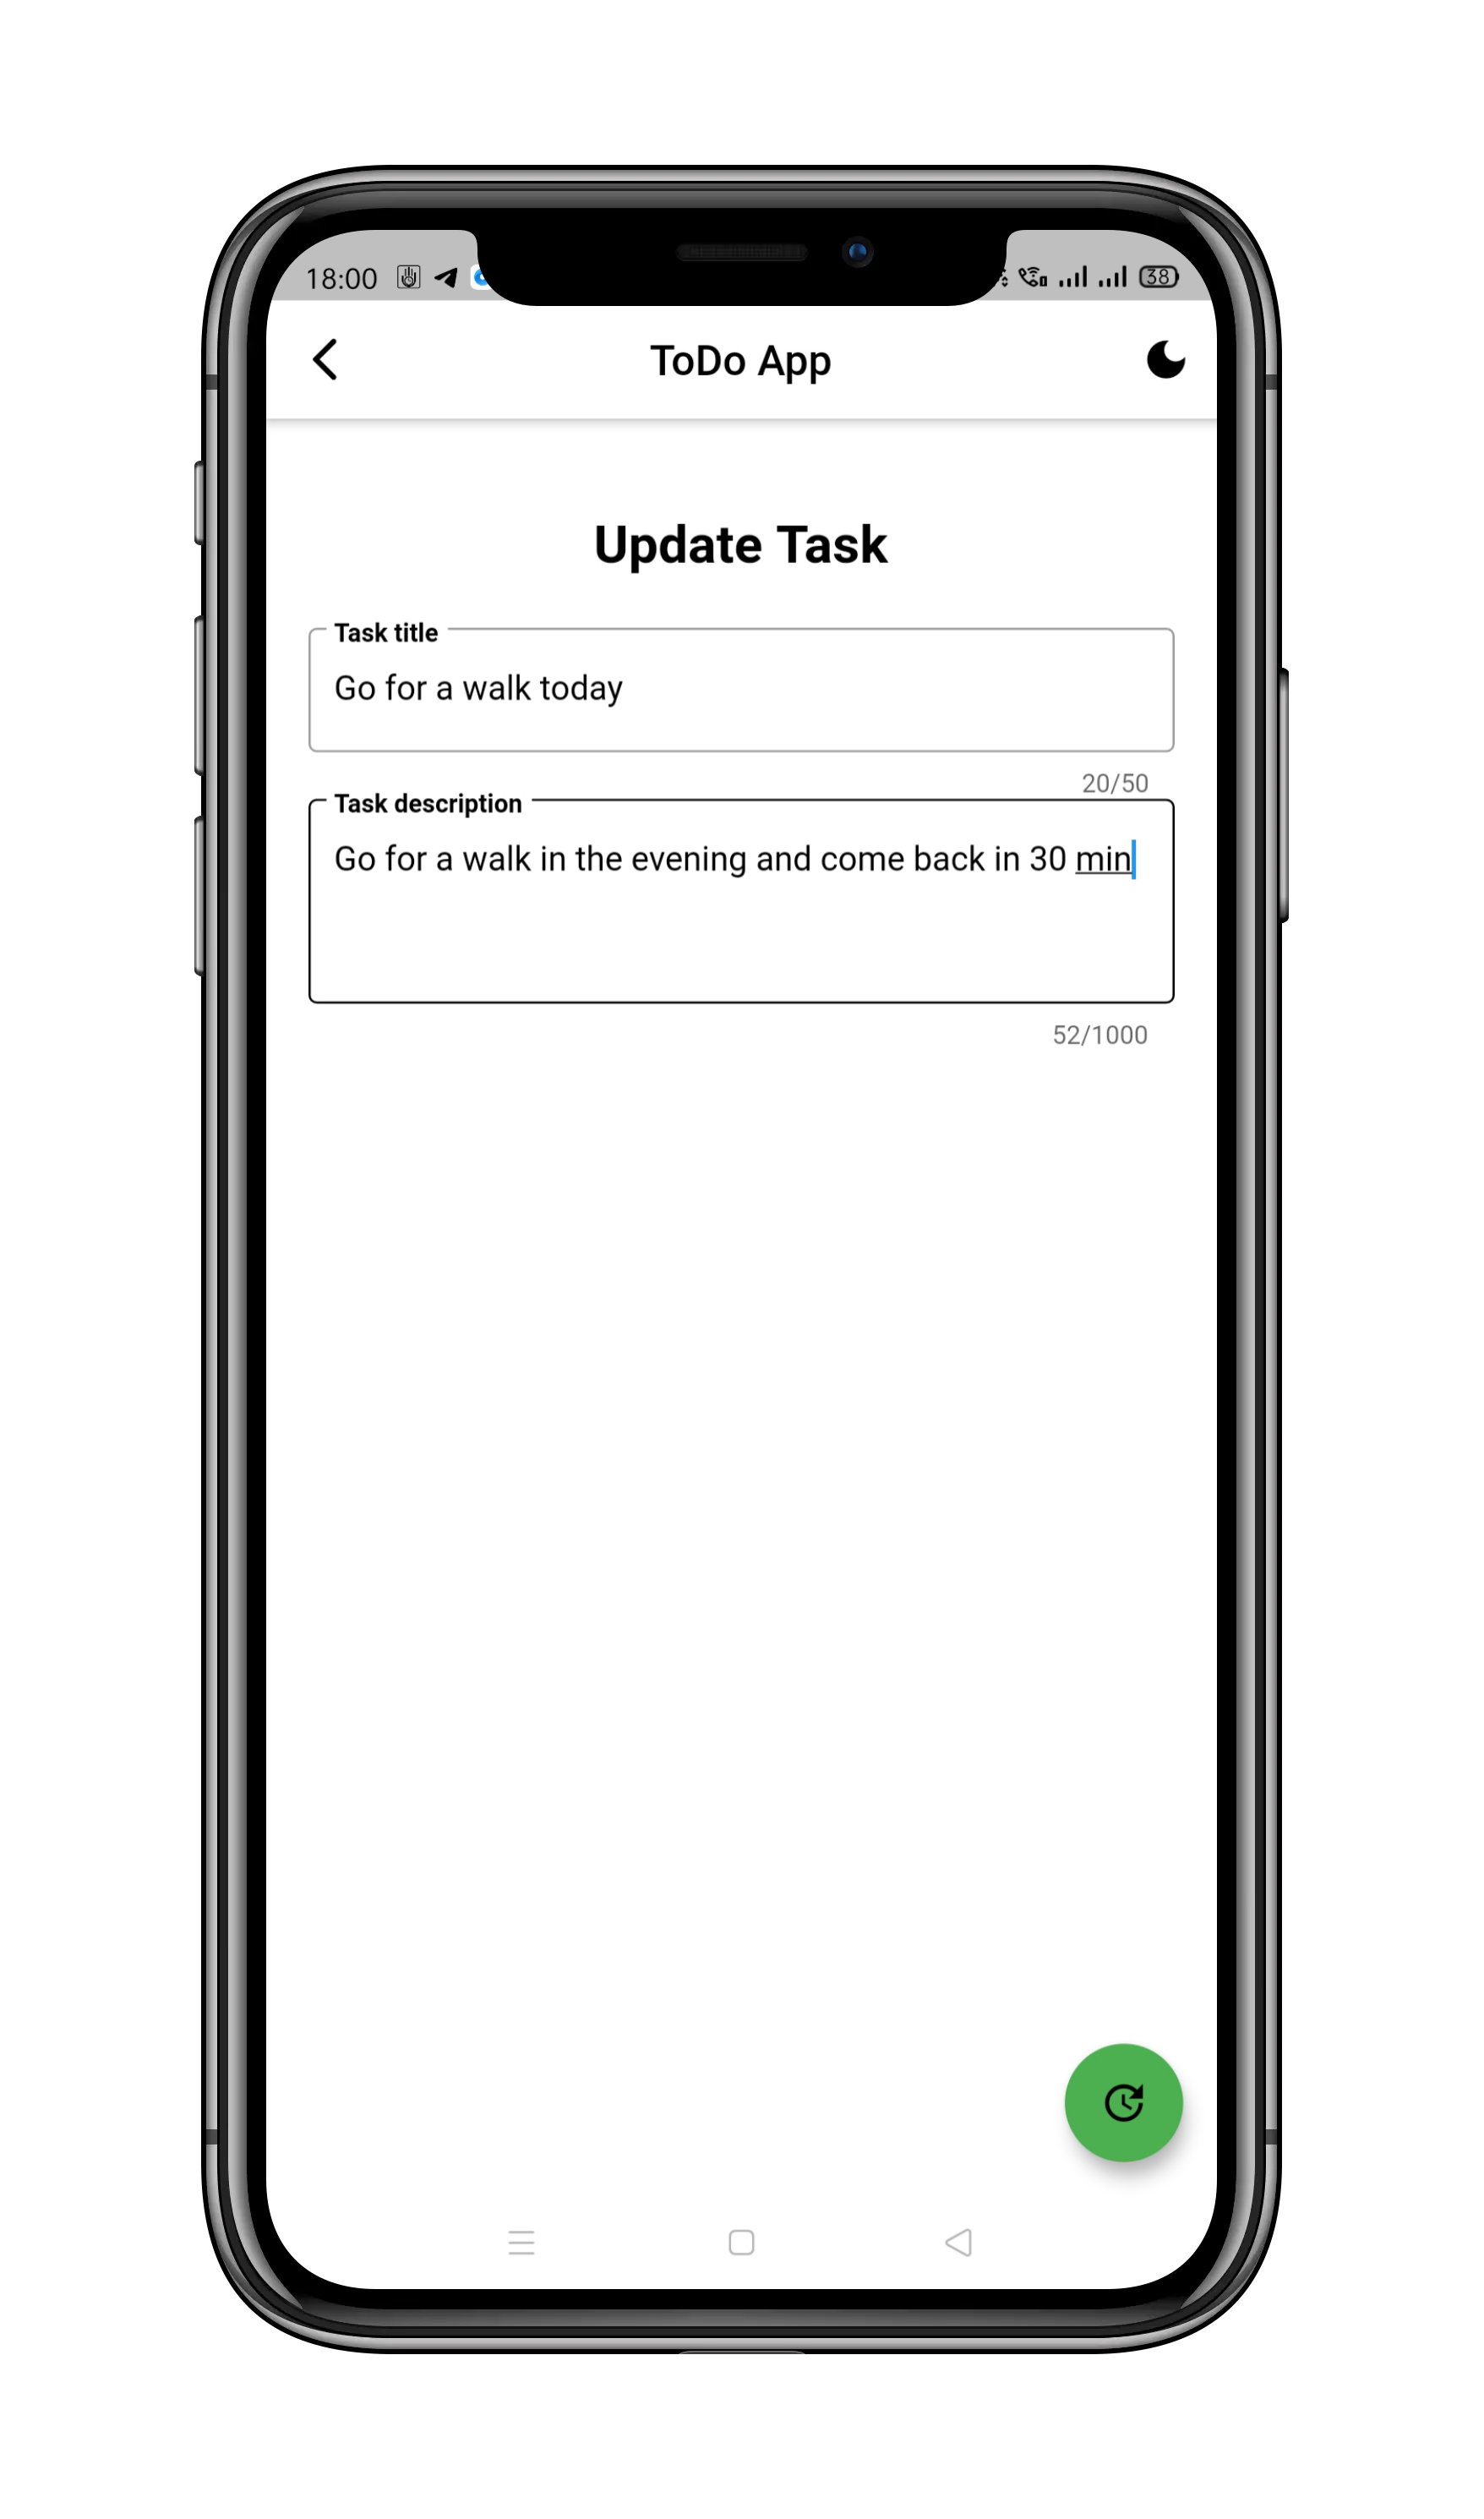
\includegraphics[height=90mm]{Images & Logos/theme/CH_08_Light_5.png}
%  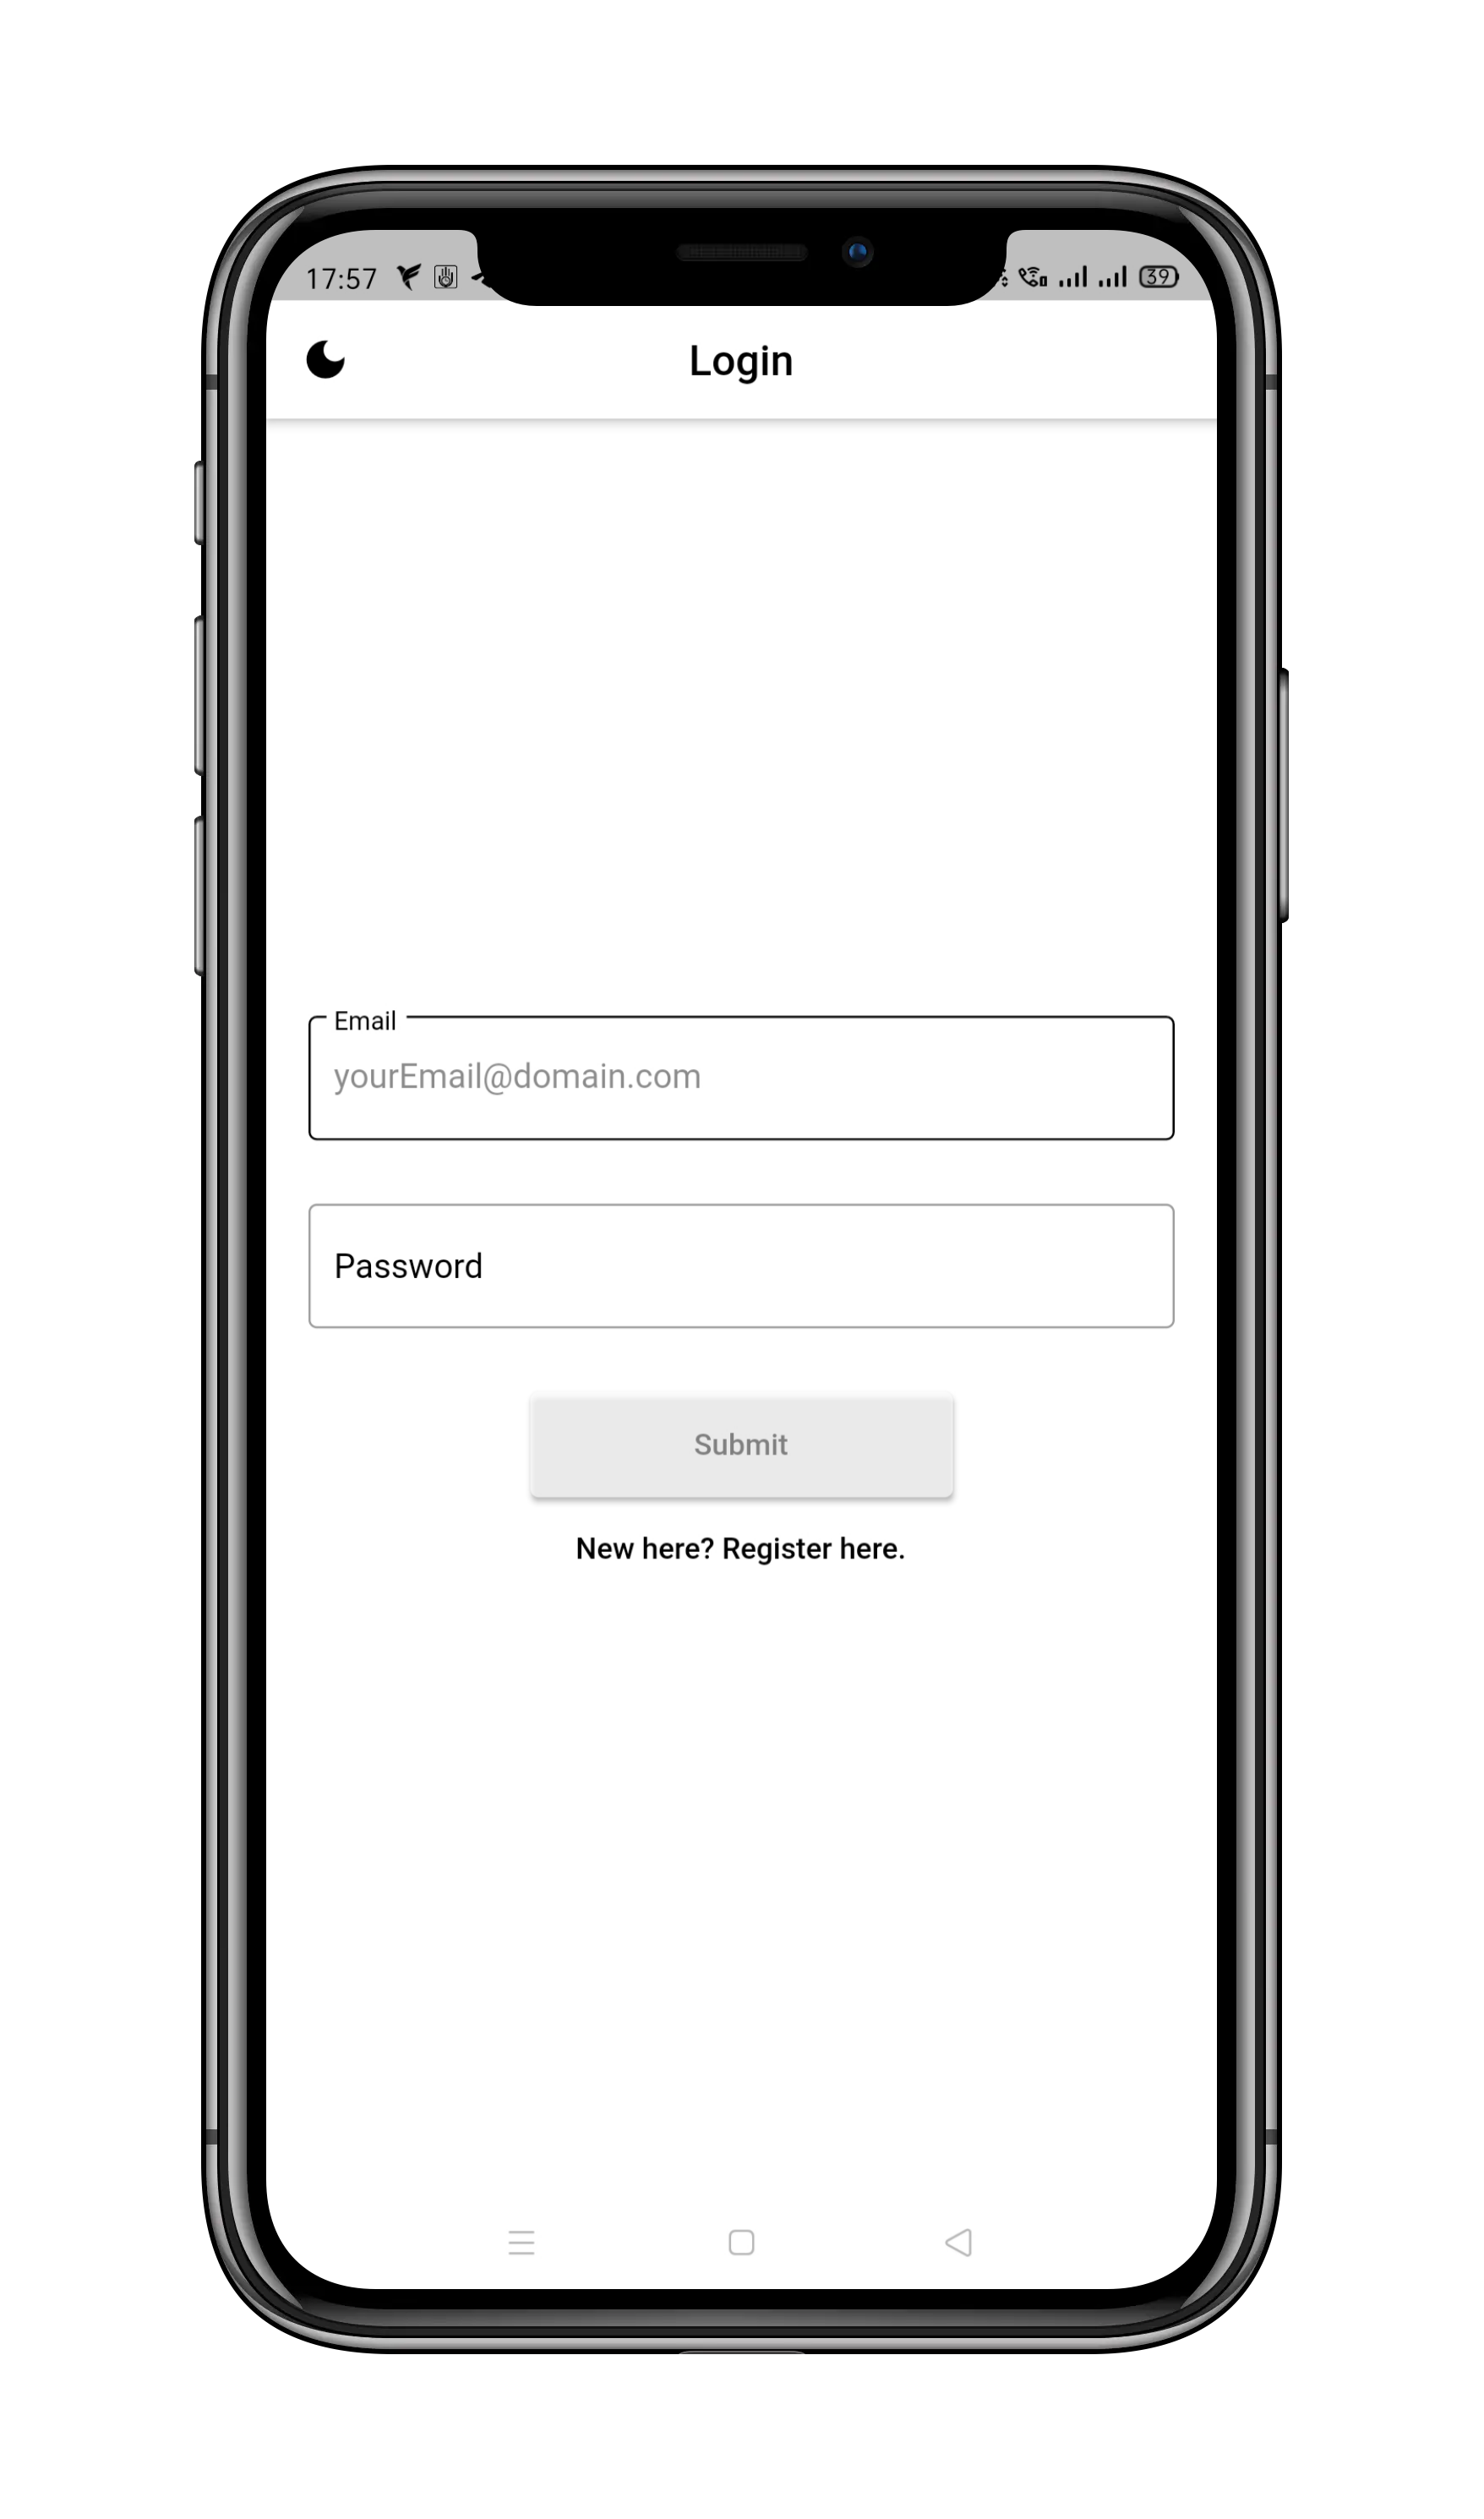
\includegraphics[height=70mm]{Images & Logos/theme/CH_08_Light_1.png}\\
%  \end{center}
%  \caption{Light Mode}
%\end{figure}  
\begin{figure}
\centering
\begin{minipage}{.5\textwidth}
  \centering
   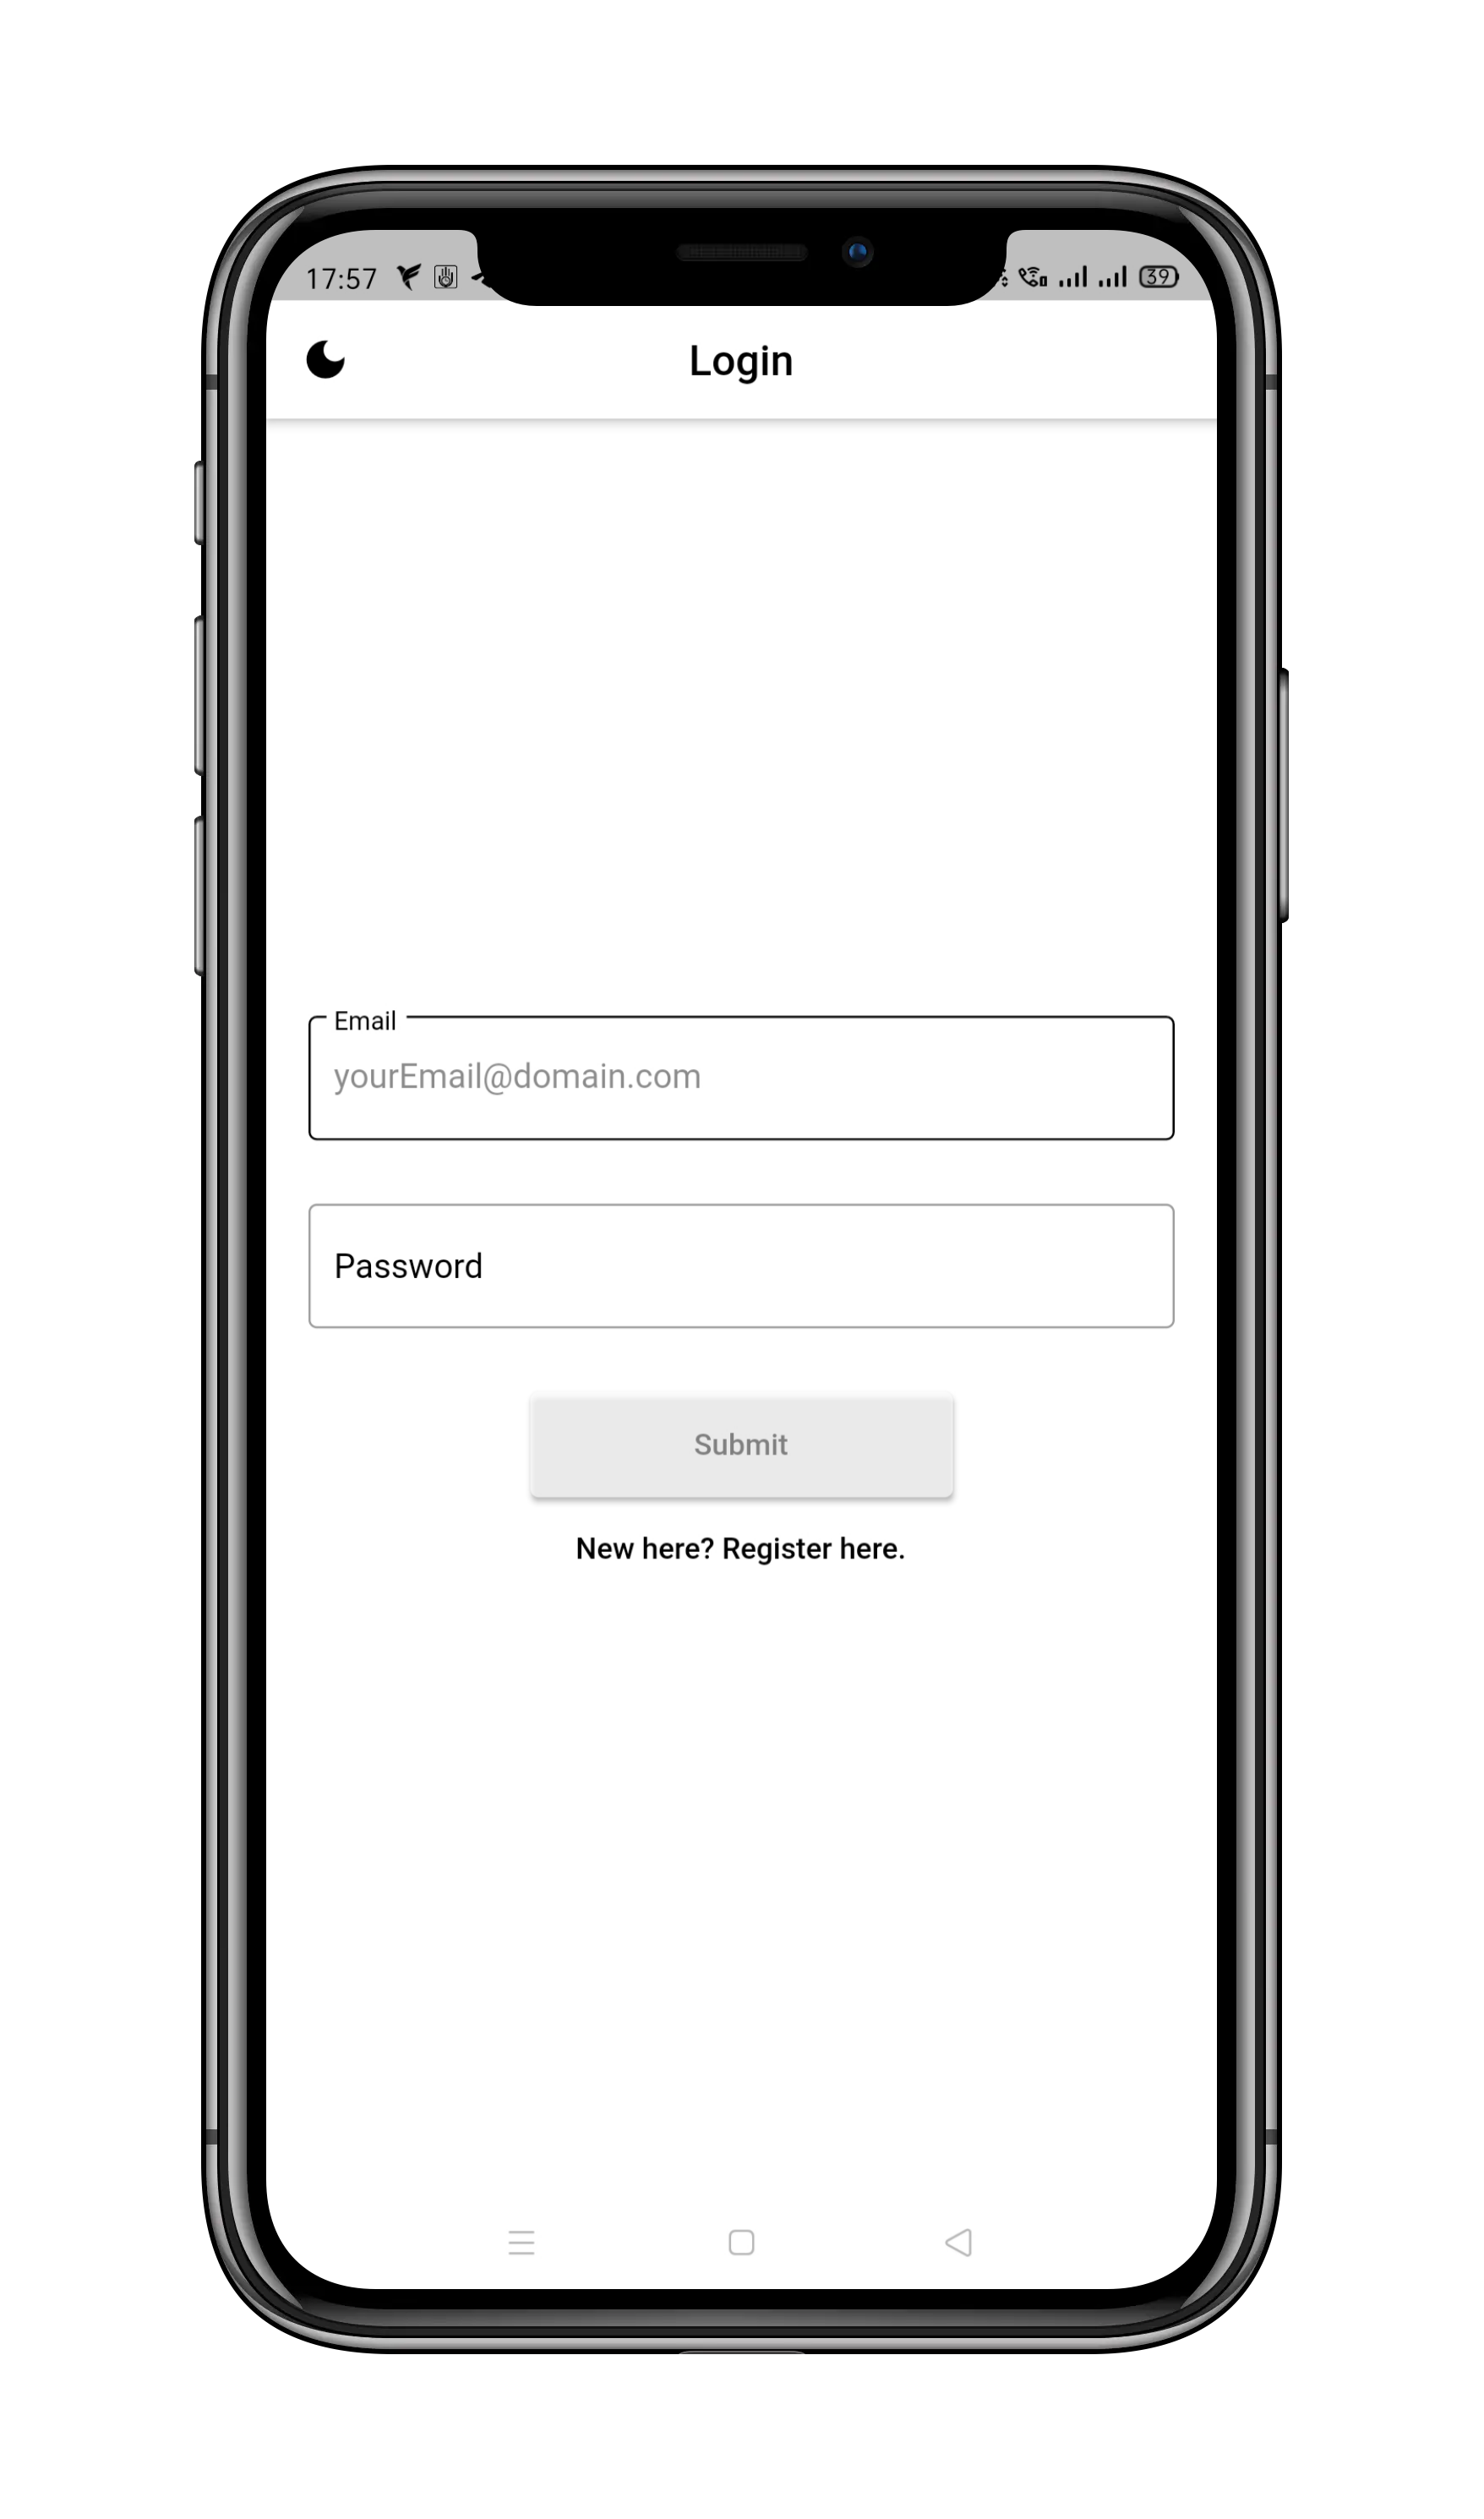
\includegraphics[height=90mm]{Images & Logos/theme/CH_08_Light_1.png}
  \caption{Login Page}
\end{minipage}%
\begin{minipage}{.5\textwidth}
  \centering
   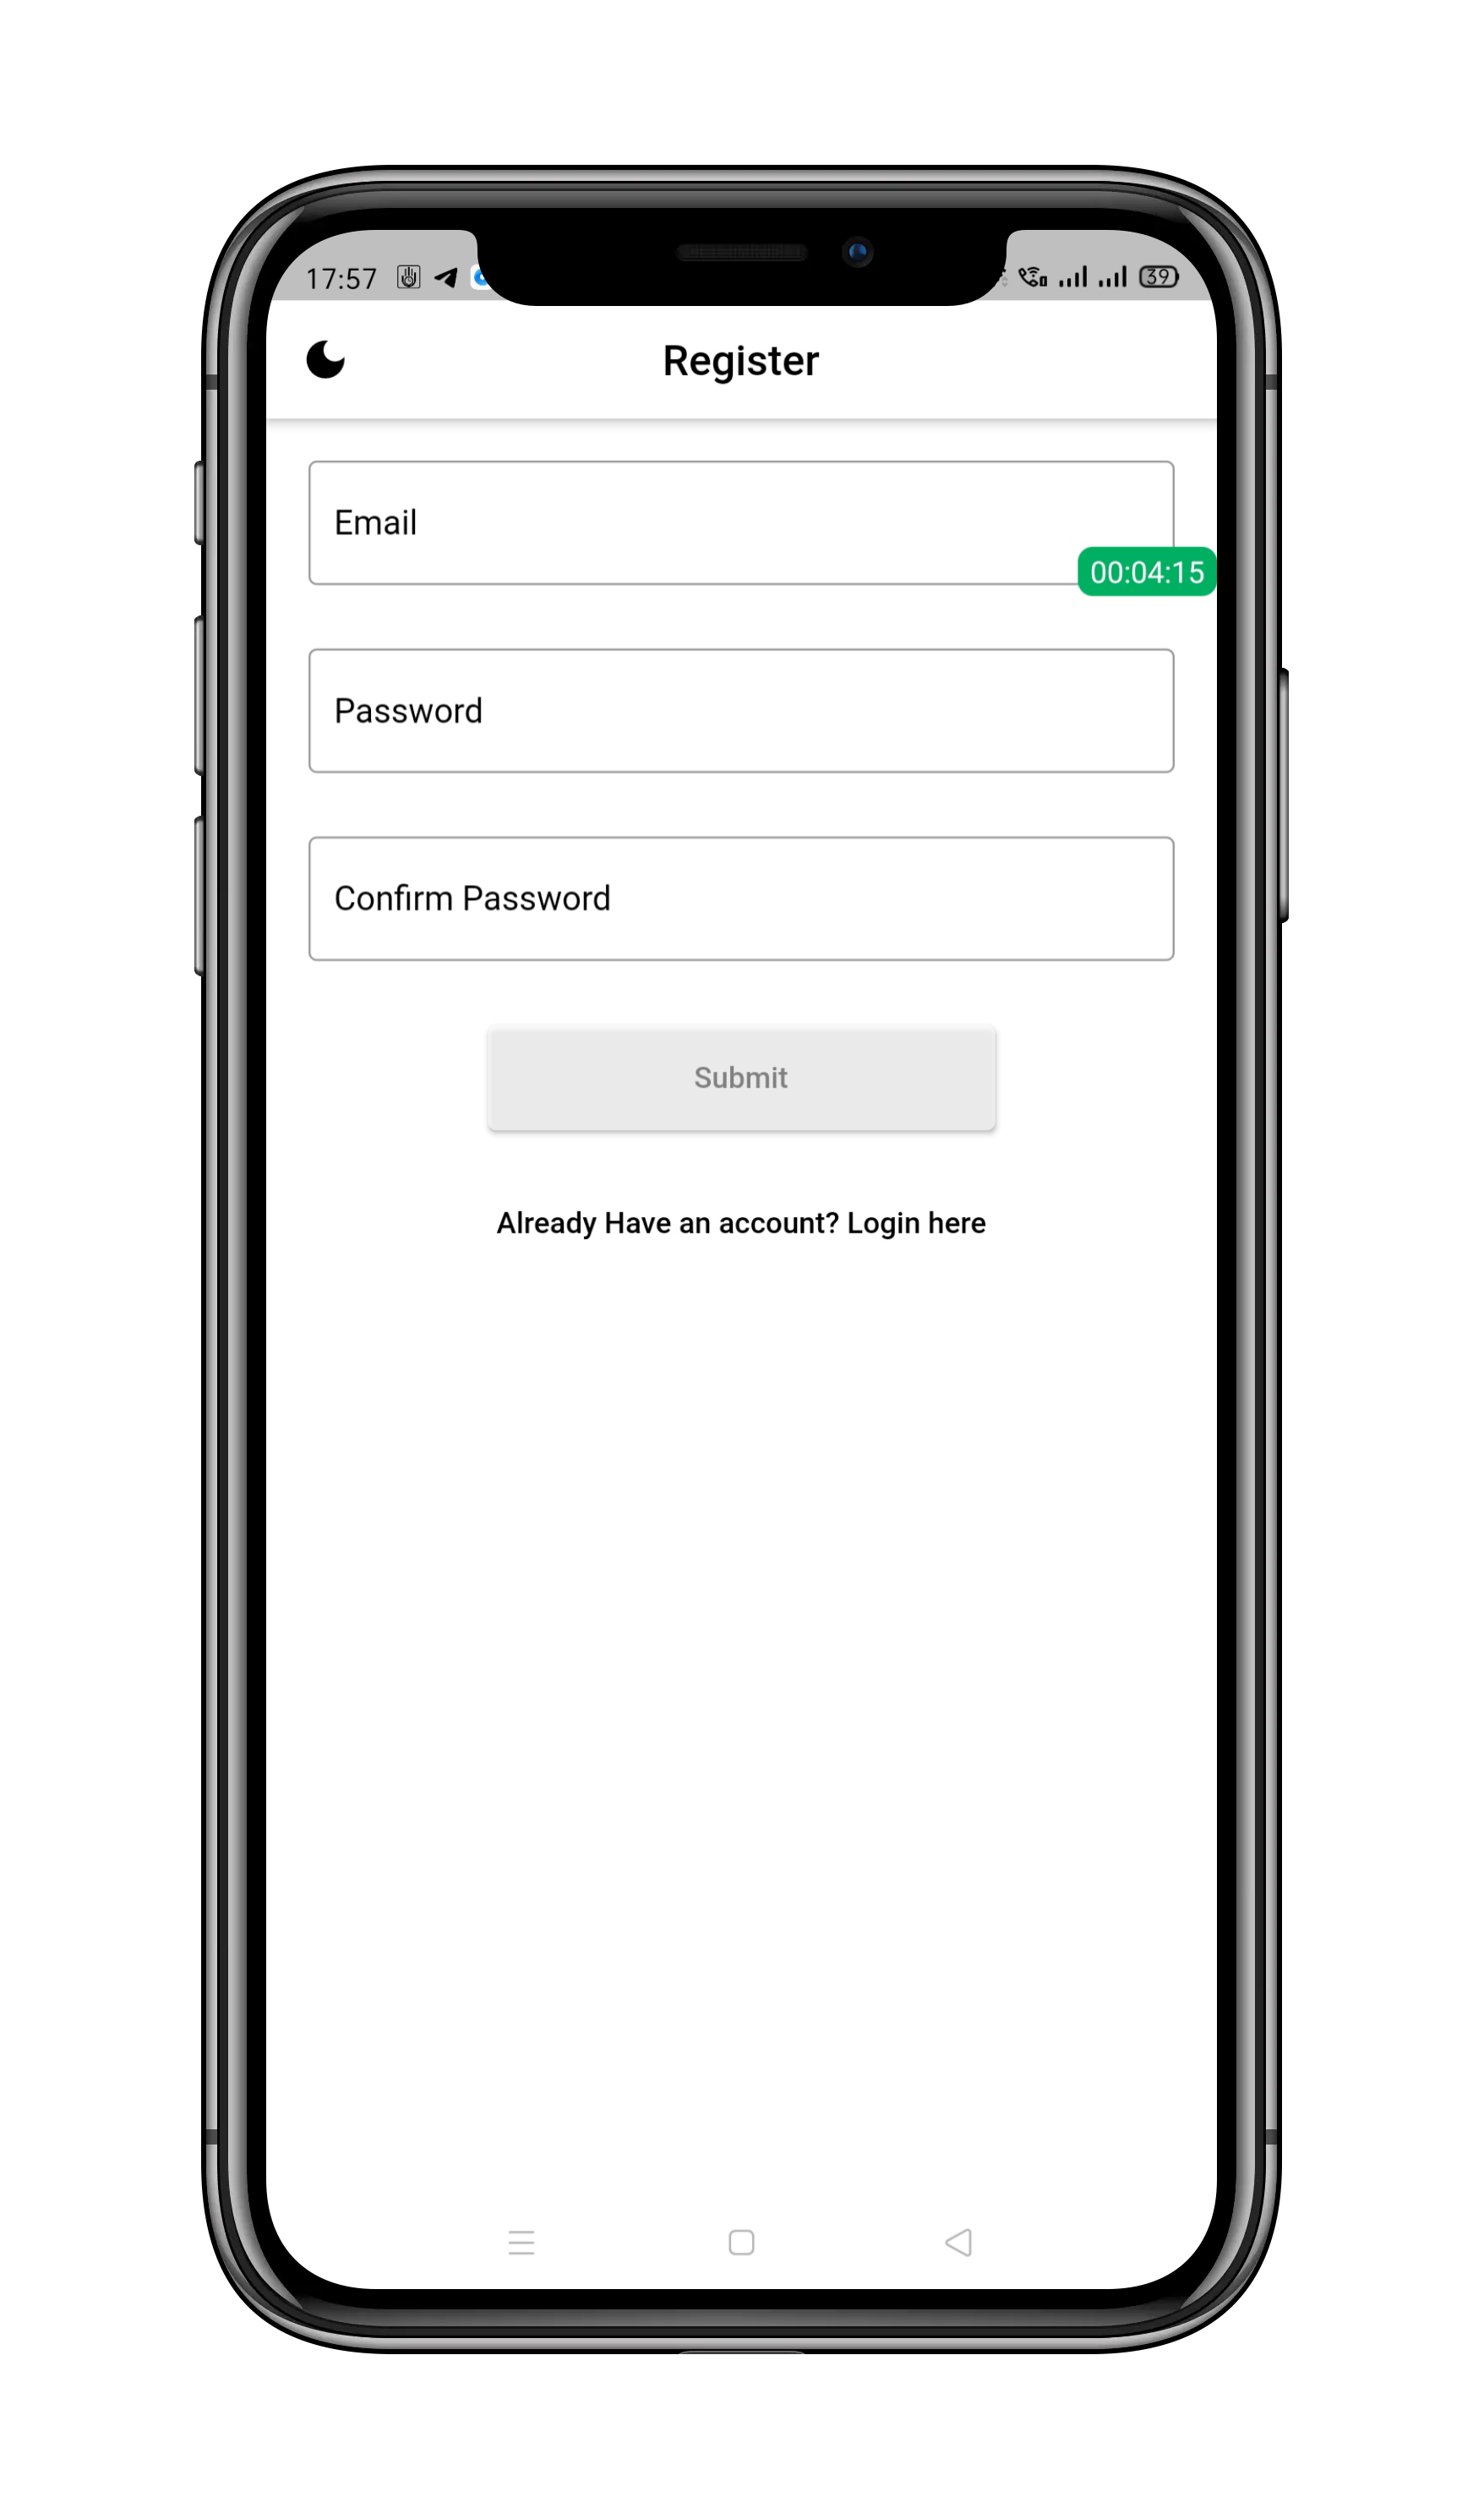
\includegraphics[height=90mm]{Images & Logos/theme/CH_08_Light_2.png}\\
  \caption{Registration page}
\end{minipage}

\centering
\begin{minipage}{.5\textwidth}
  \centering
   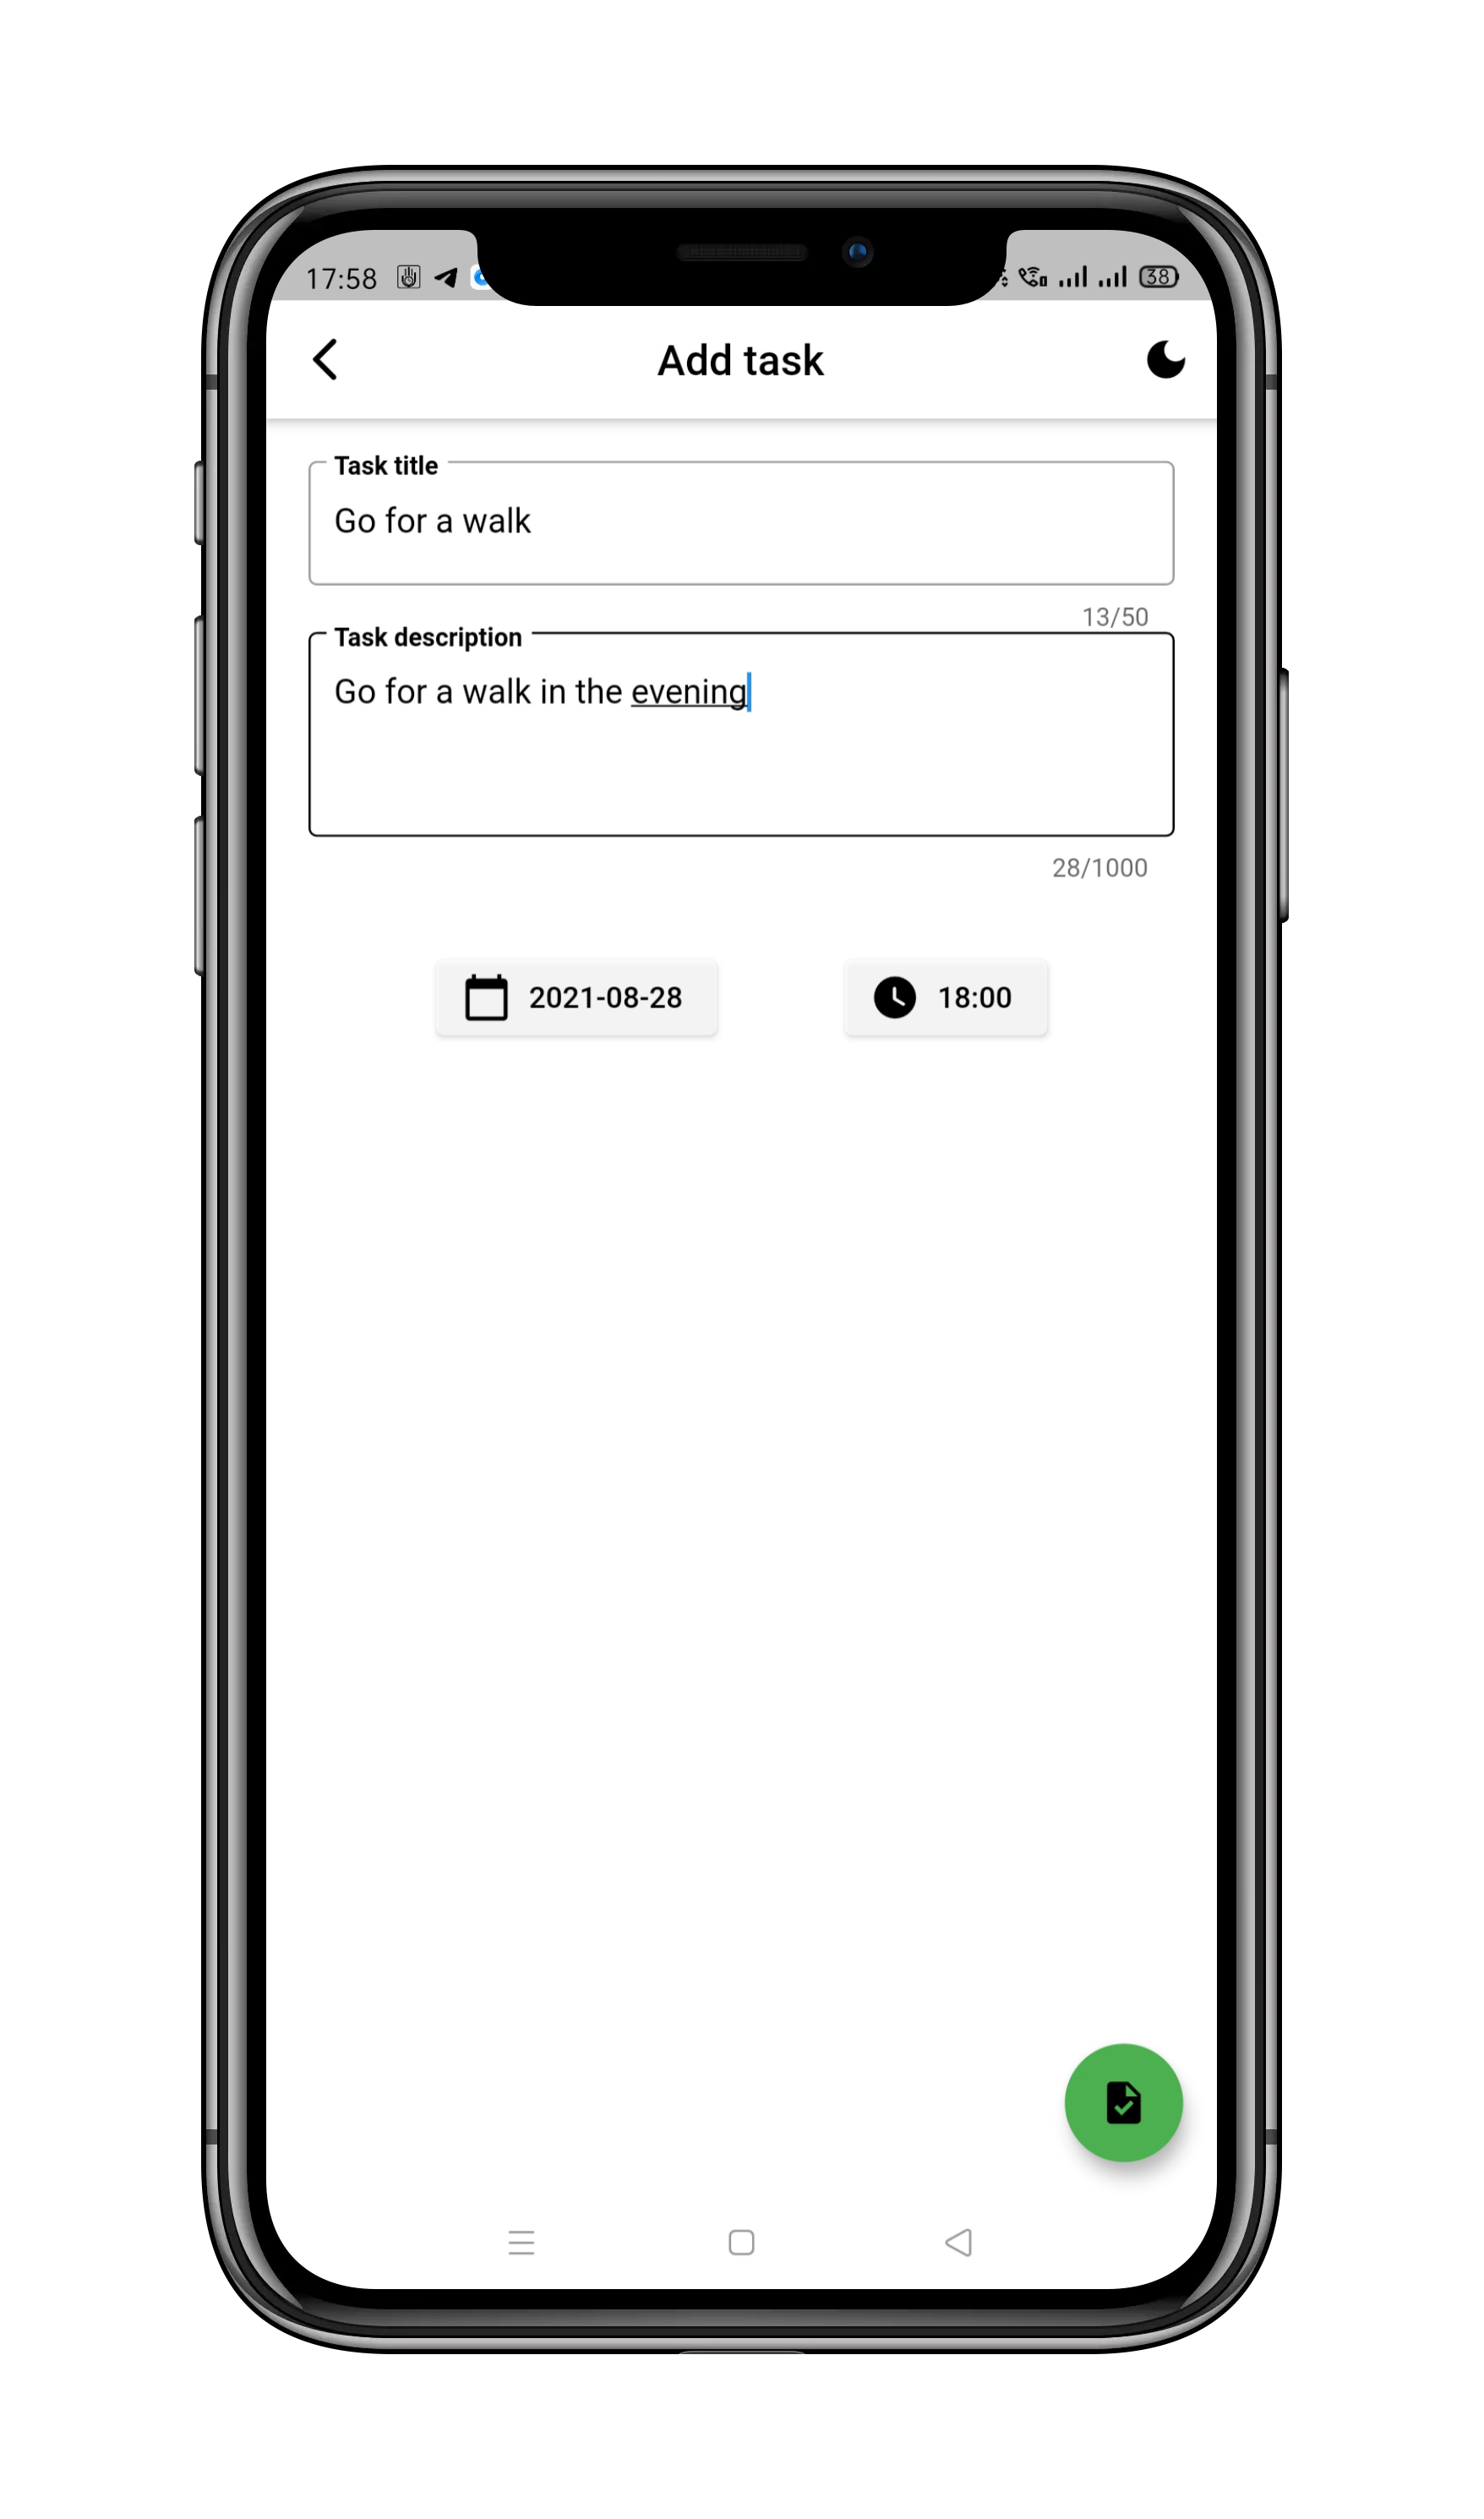
\includegraphics[height=90mm]{Images & Logos/theme/CH_08_Light_3.png}
  \caption{Add Task Page}
\end{minipage}%
\begin{minipage}{.5\textwidth}
  \centering
   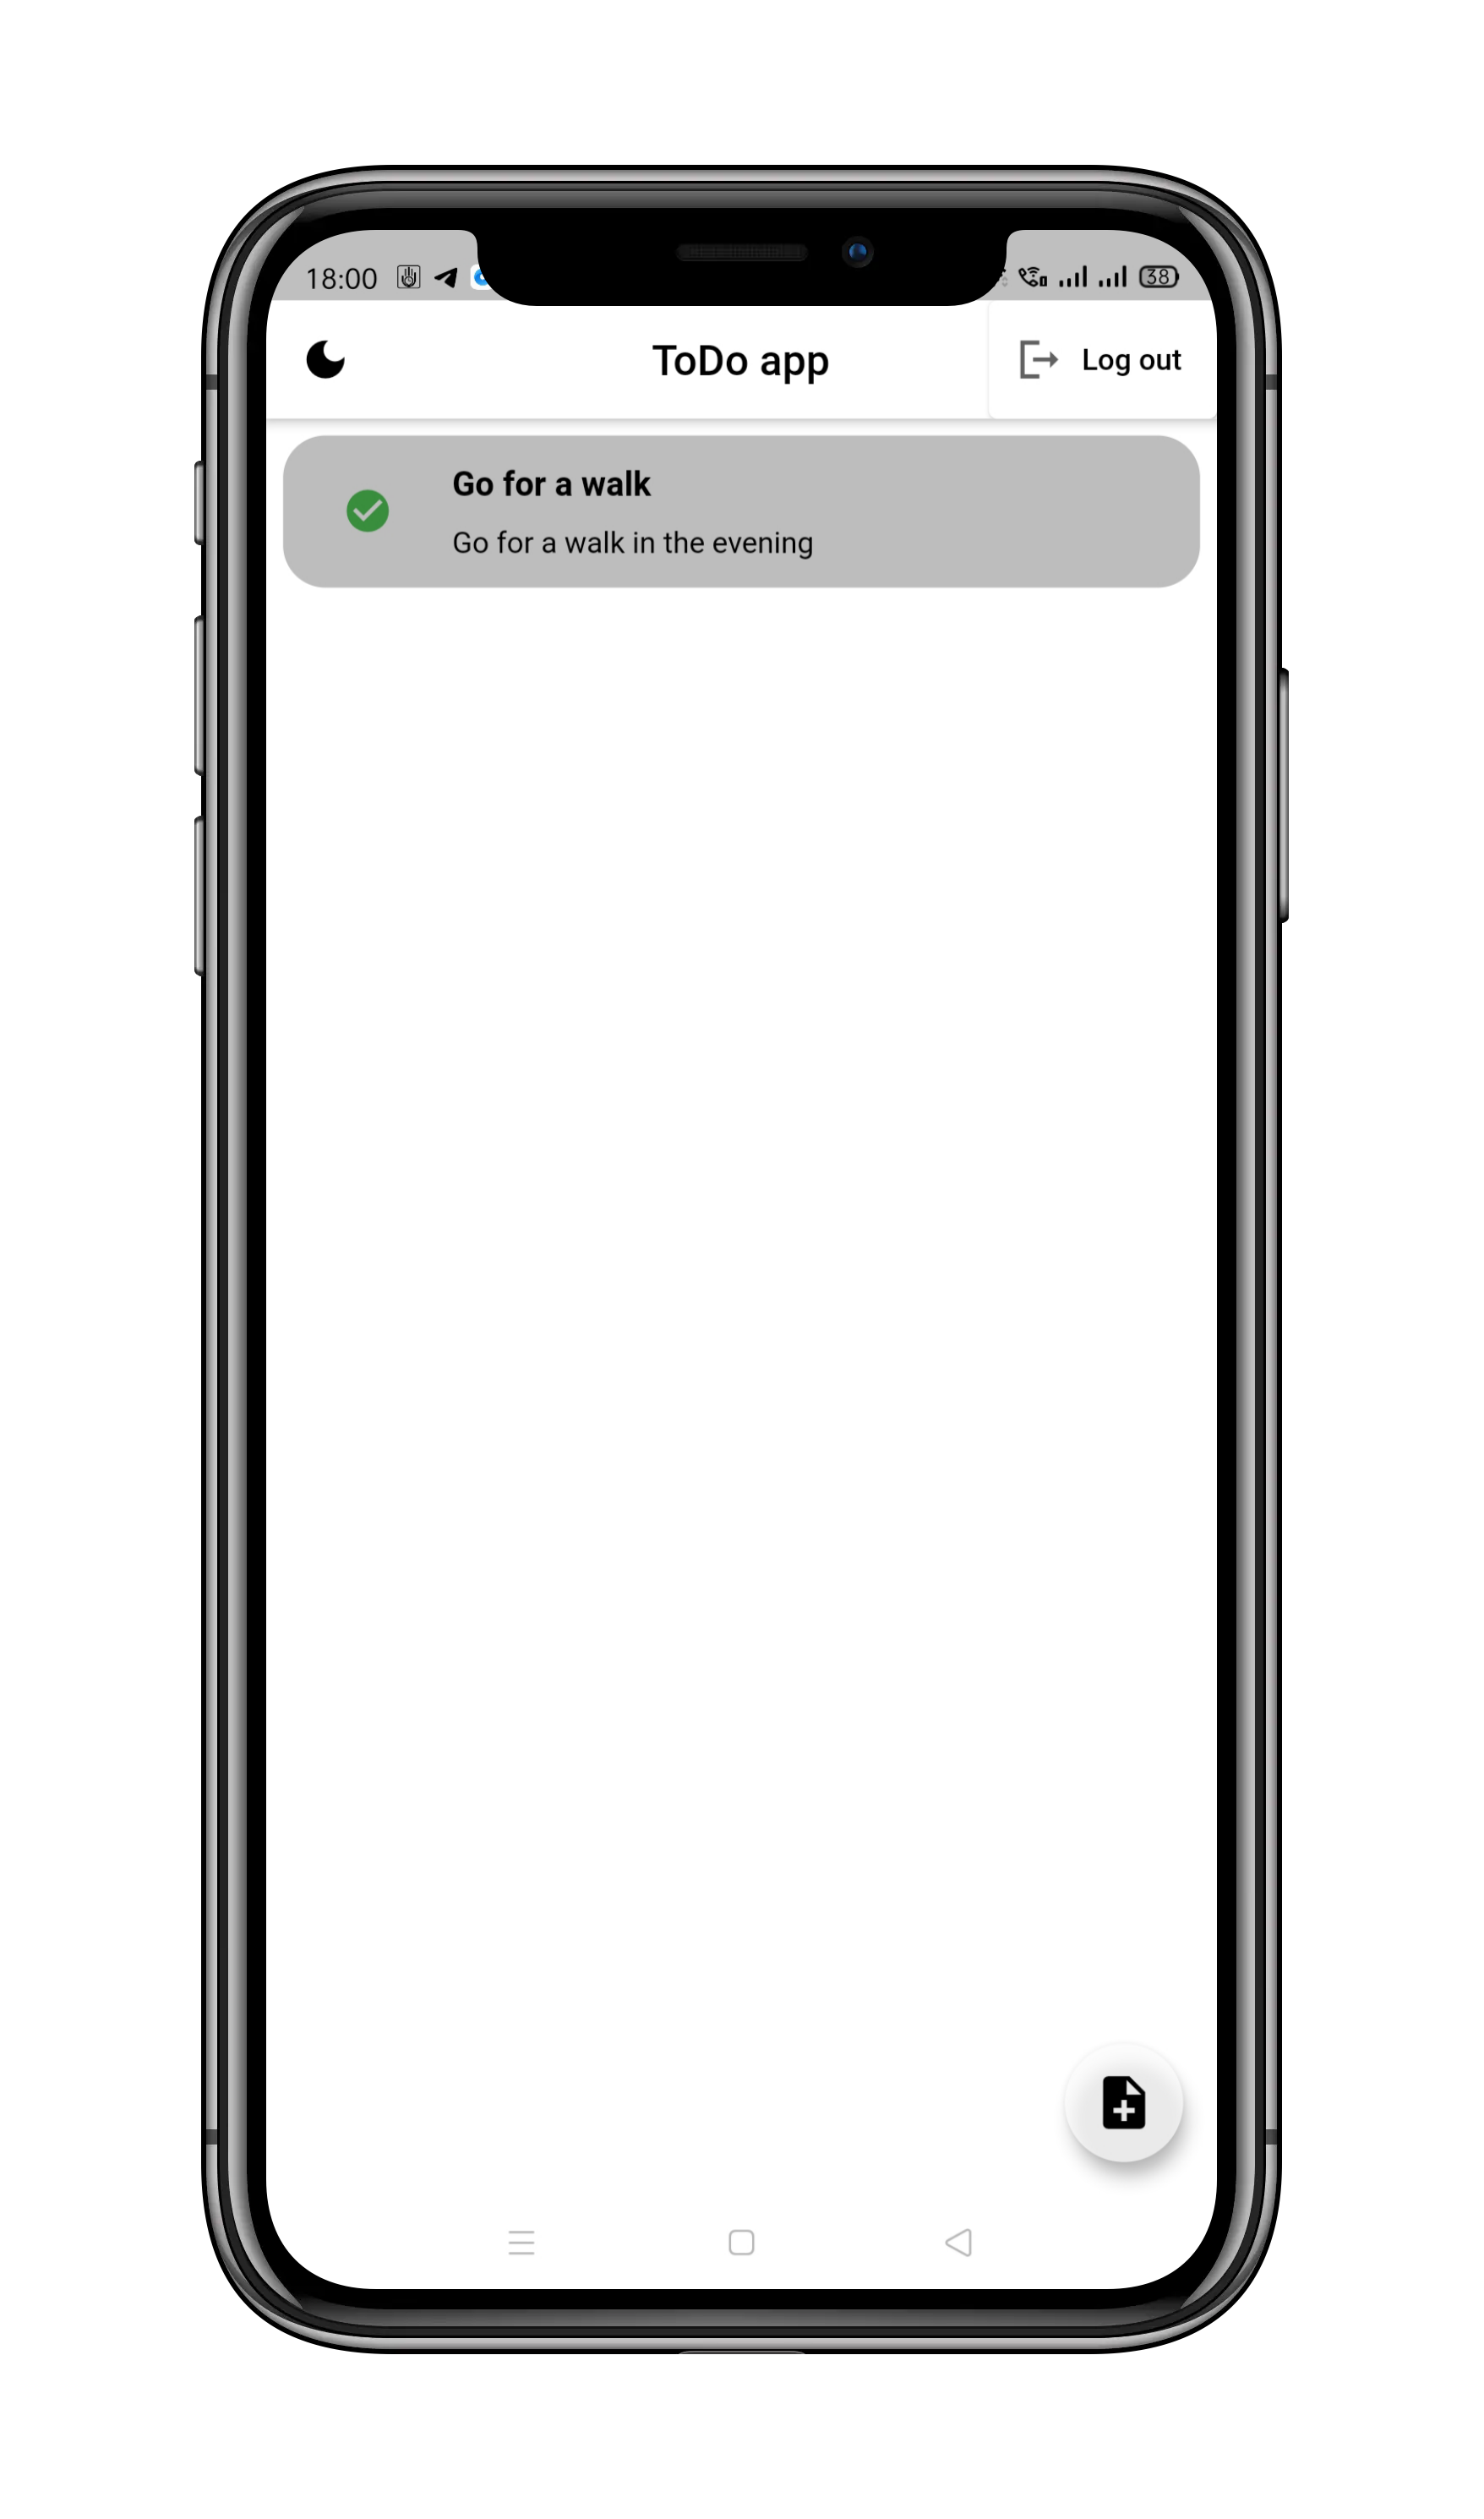
\includegraphics[height=90mm]{Images & Logos/theme/CH_08_Light_4.png}
  \caption{Home page}
\end{minipage}
\newpage
\end{figure}

\begin{figure}[h]
  \begin{center}
   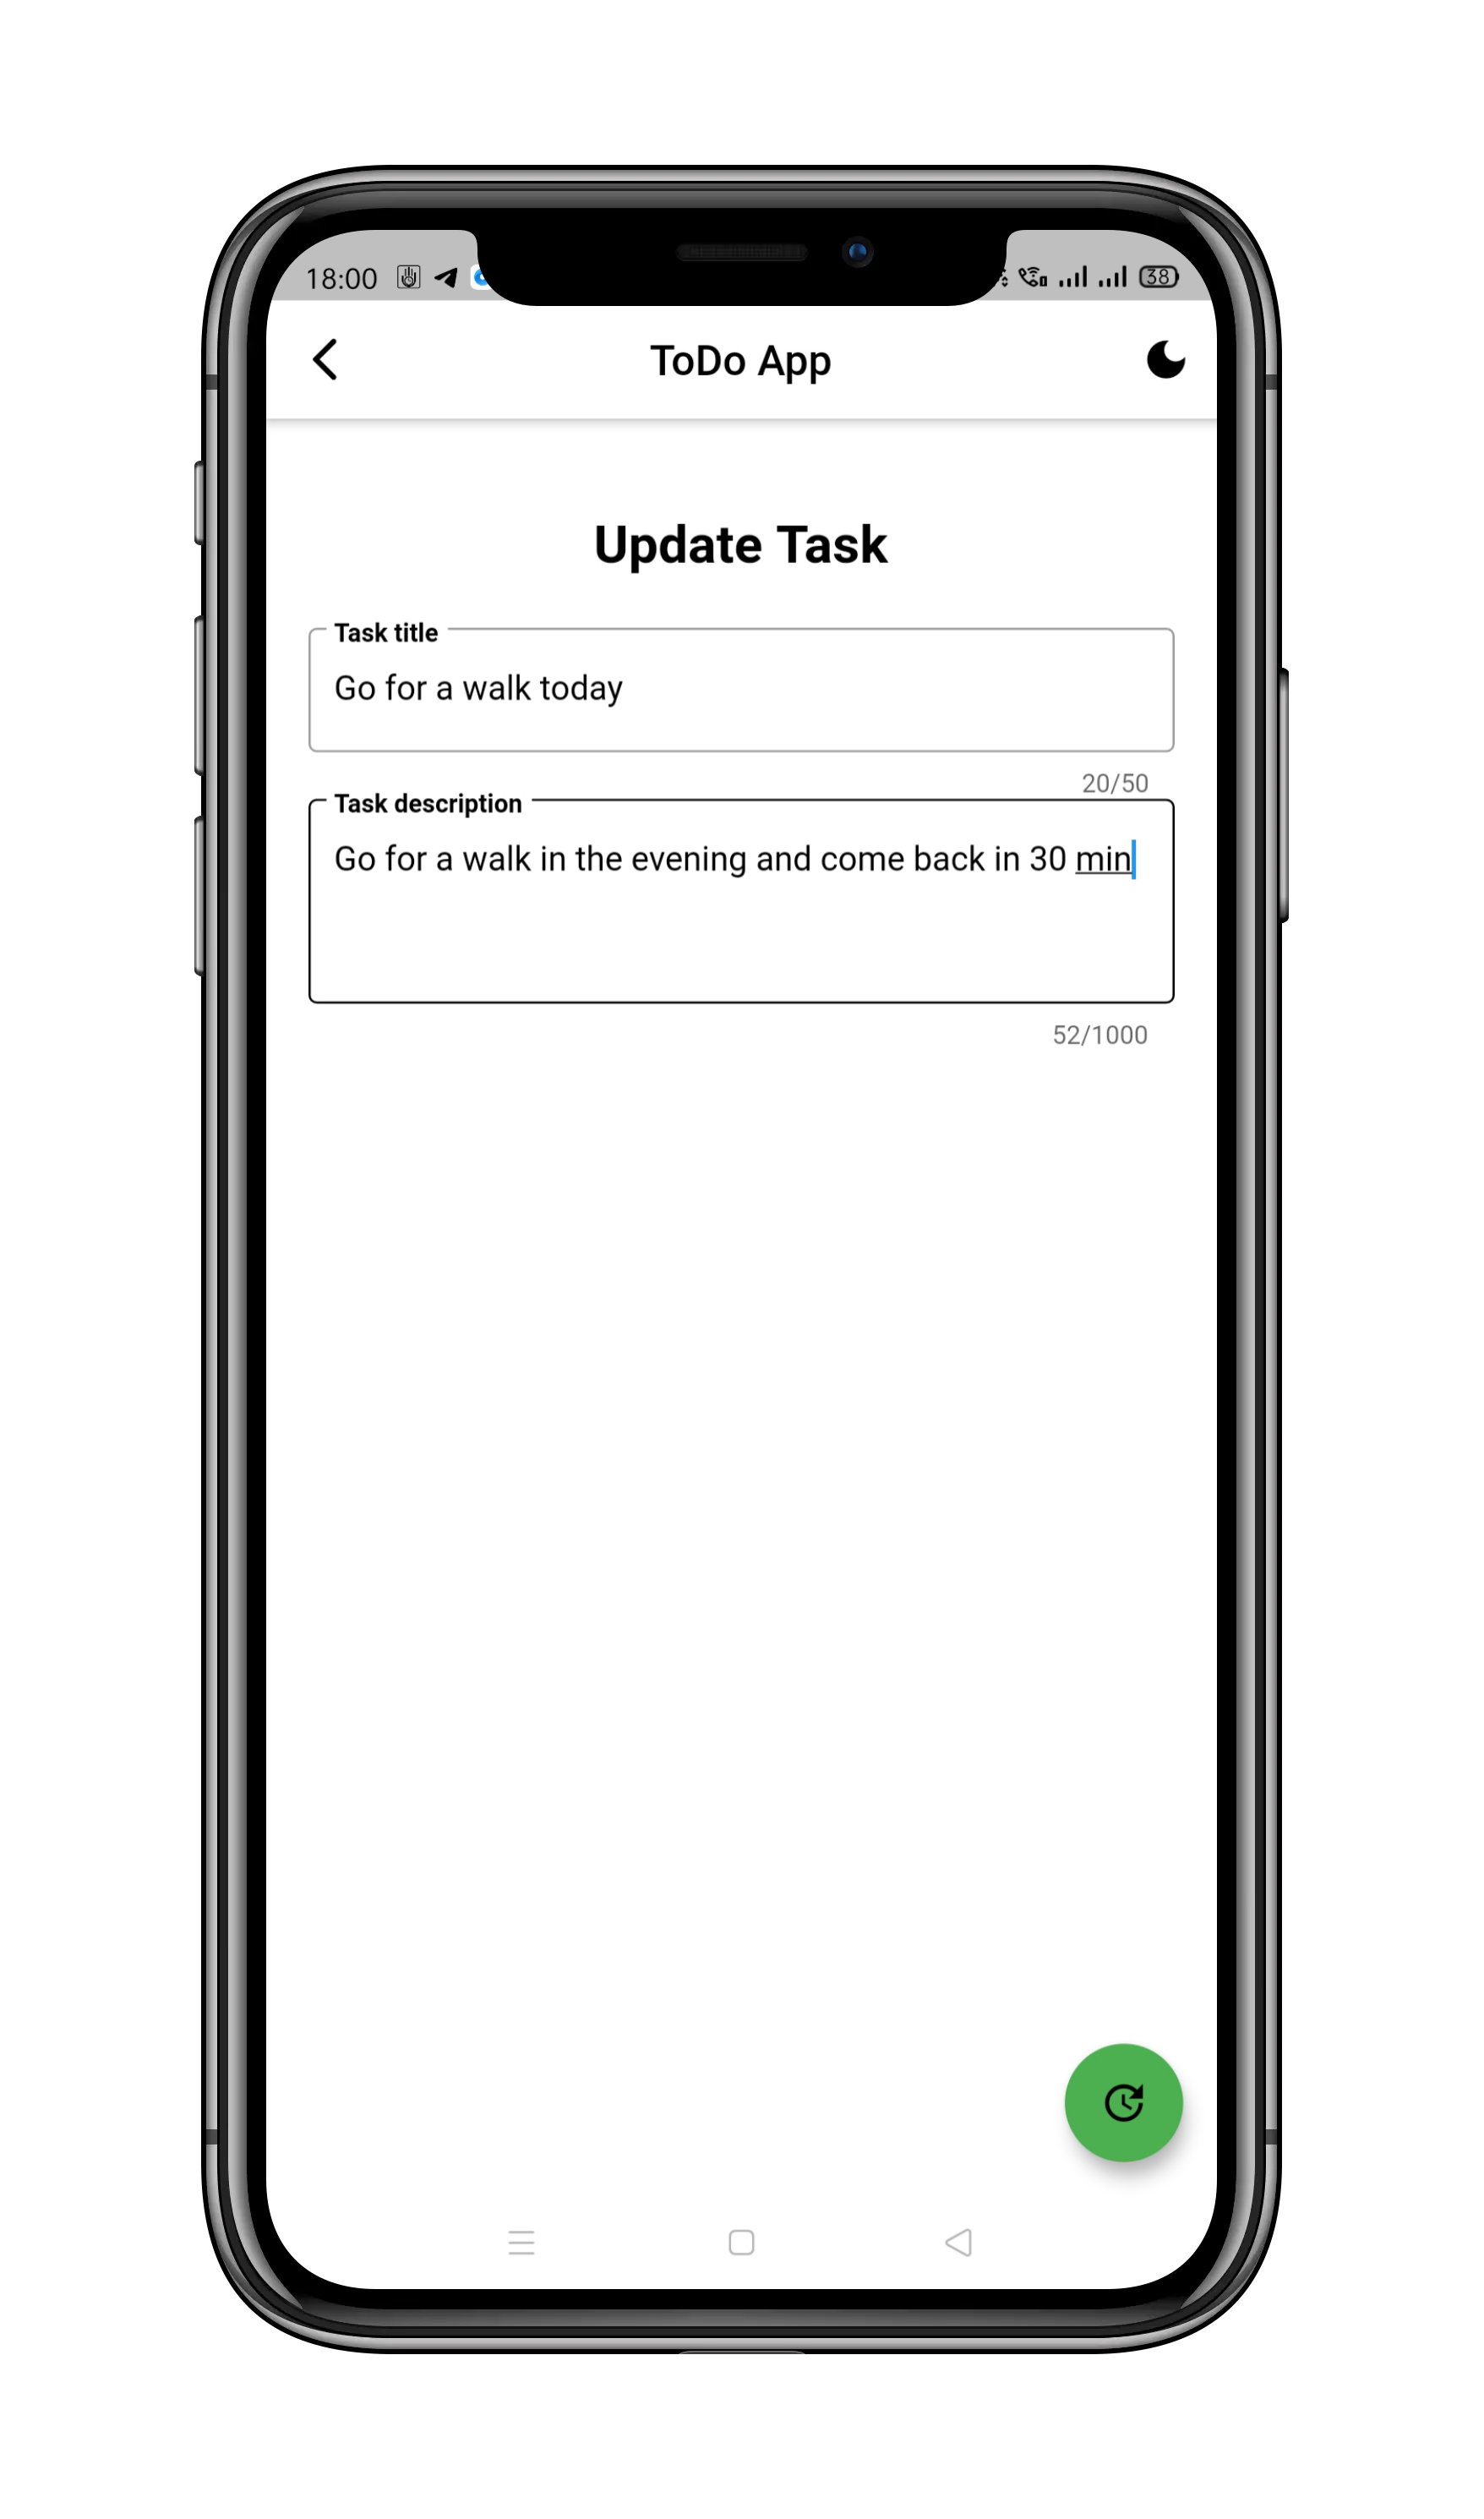
\includegraphics[height=90mm]{Images & Logos/theme/CH_08_Light_5.png}
%  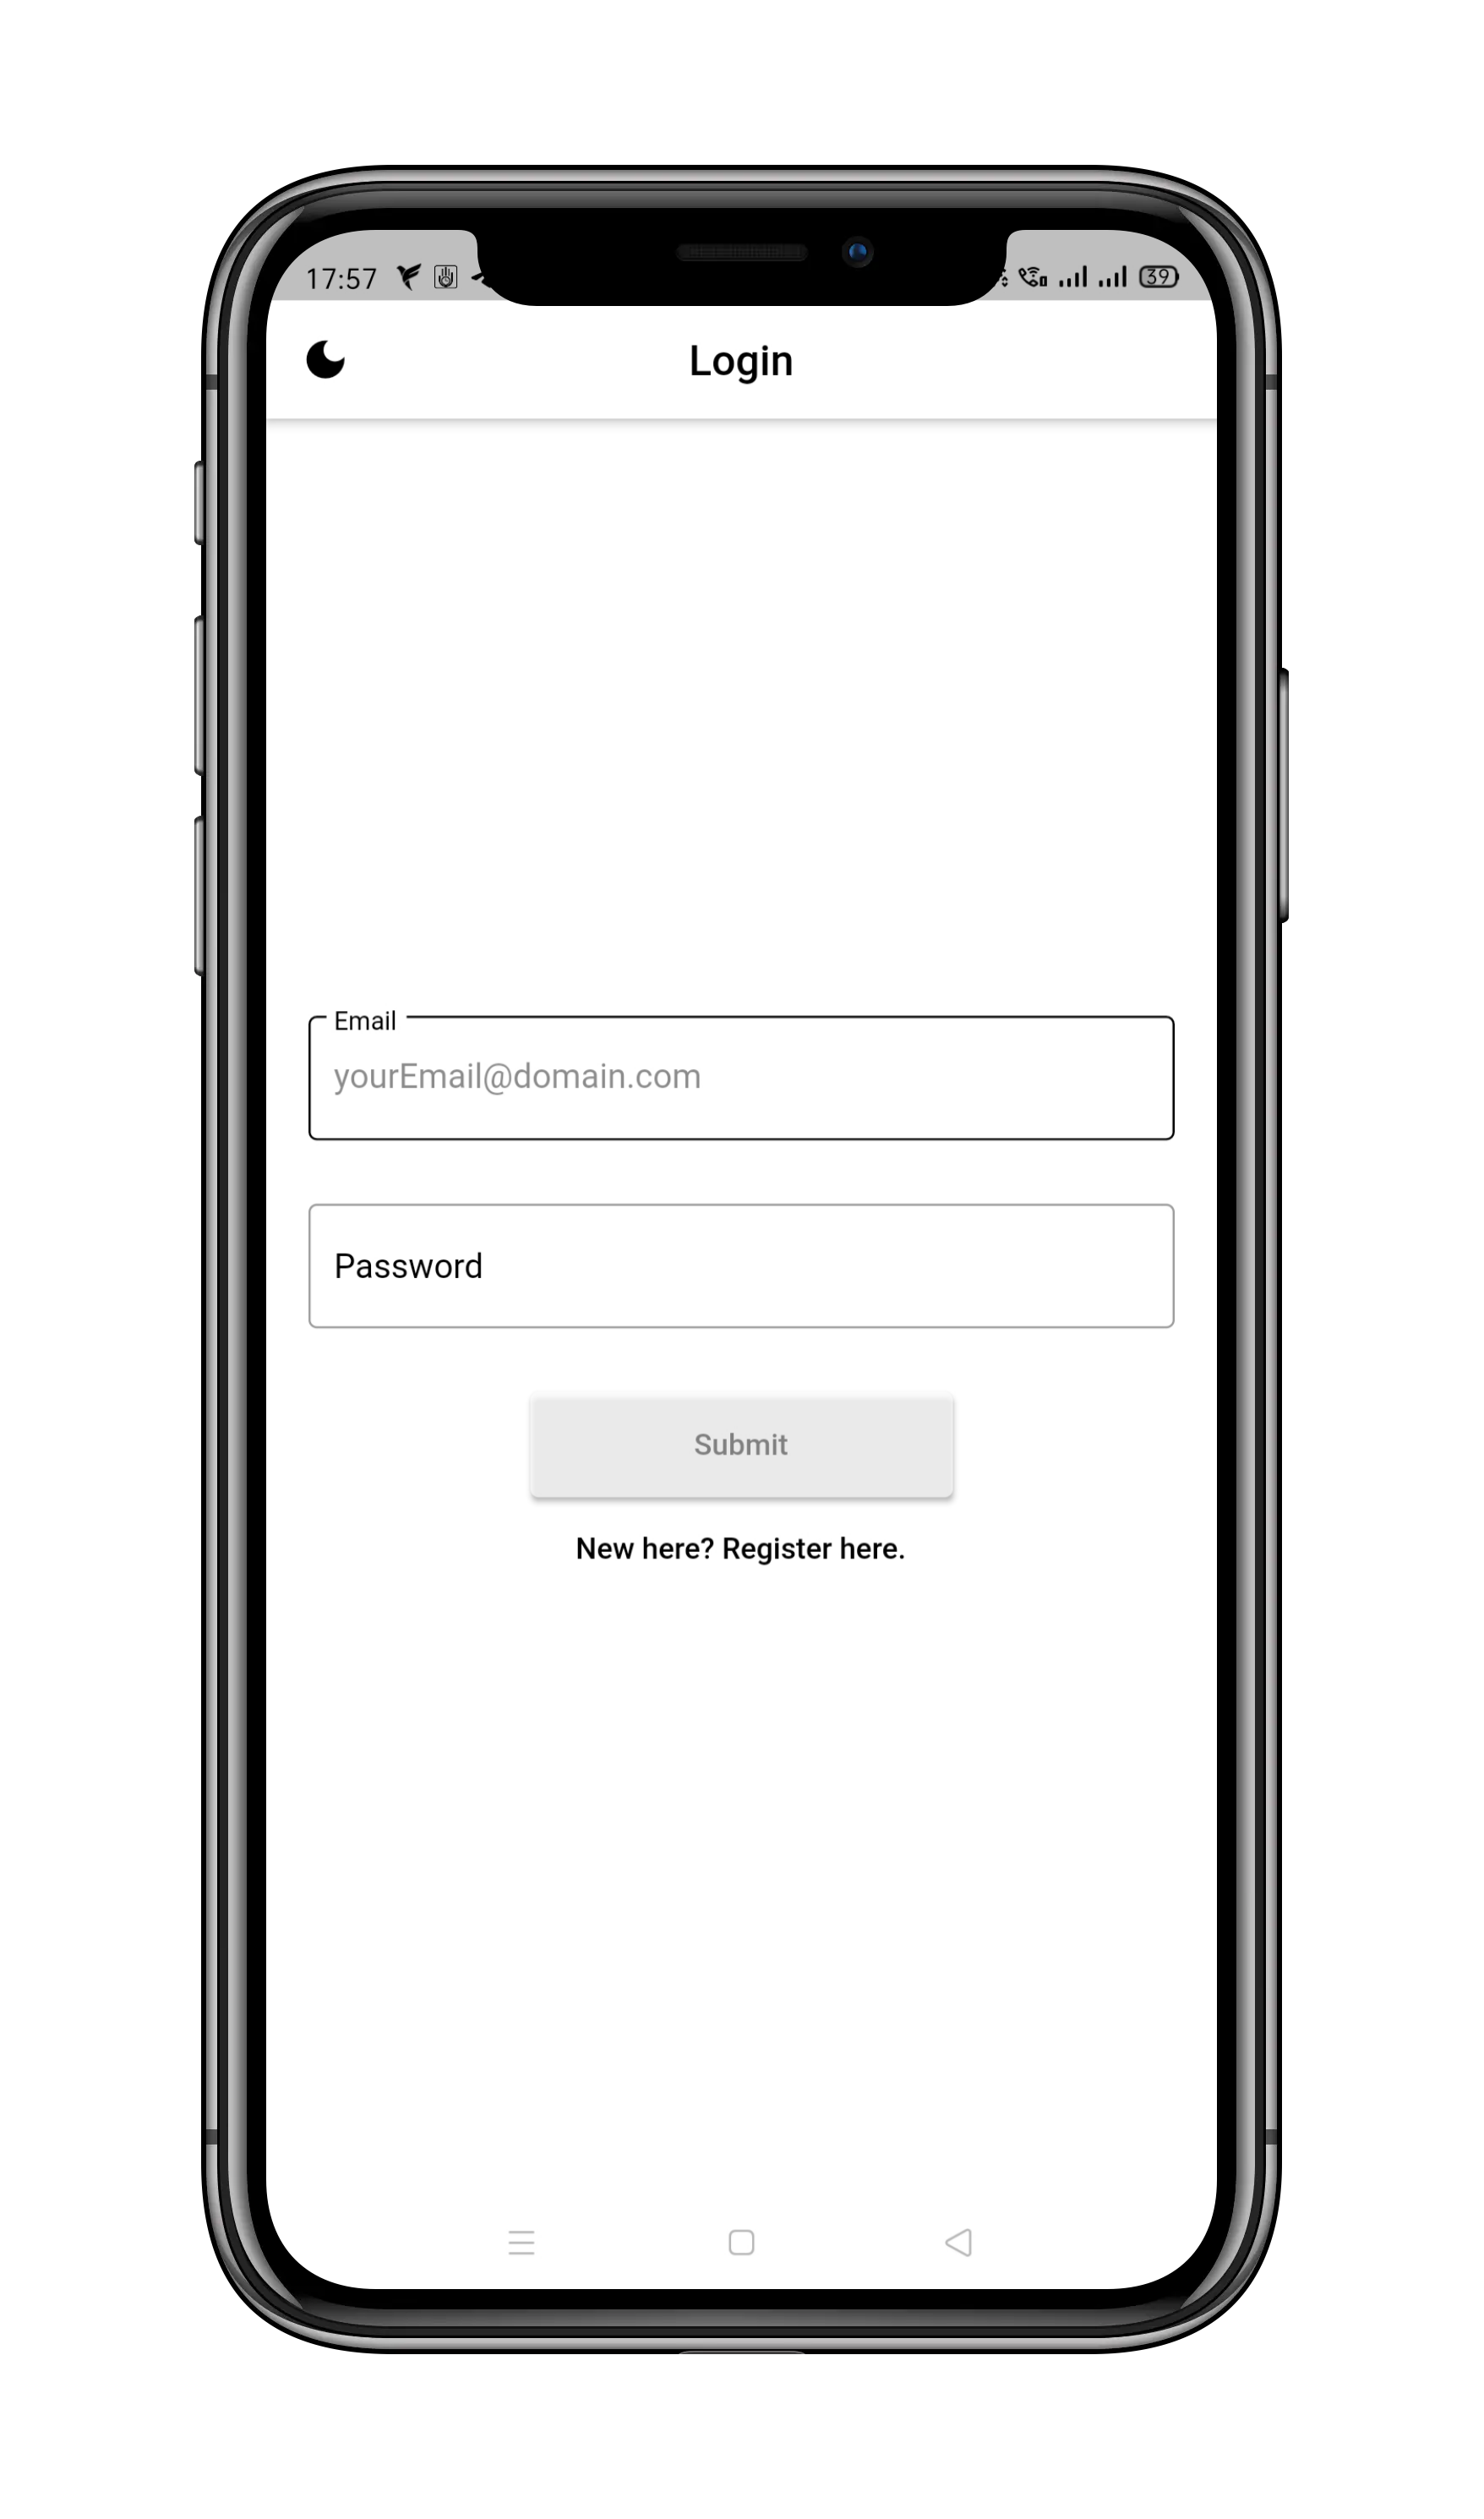
\includegraphics[height=70mm]{Images & Logos/theme/CH_08_Light_1.png}\\
  \end{center}
  \caption{Update Task Page}
\end{figure}  
\newpage
\hfill
\subsection{Dark Mode}
\begin{itemize}
\item An eye friendly shade of black as background of app (Hexcode: \#1A1A1A)
\item Black buttons with a silver-white outline
\item White icons
\item Green add task icon
\item Yellow color edit task icon
\end{itemize}

\begin{figure}
\centering
\begin{minipage}{.5\textwidth}
  \centering
   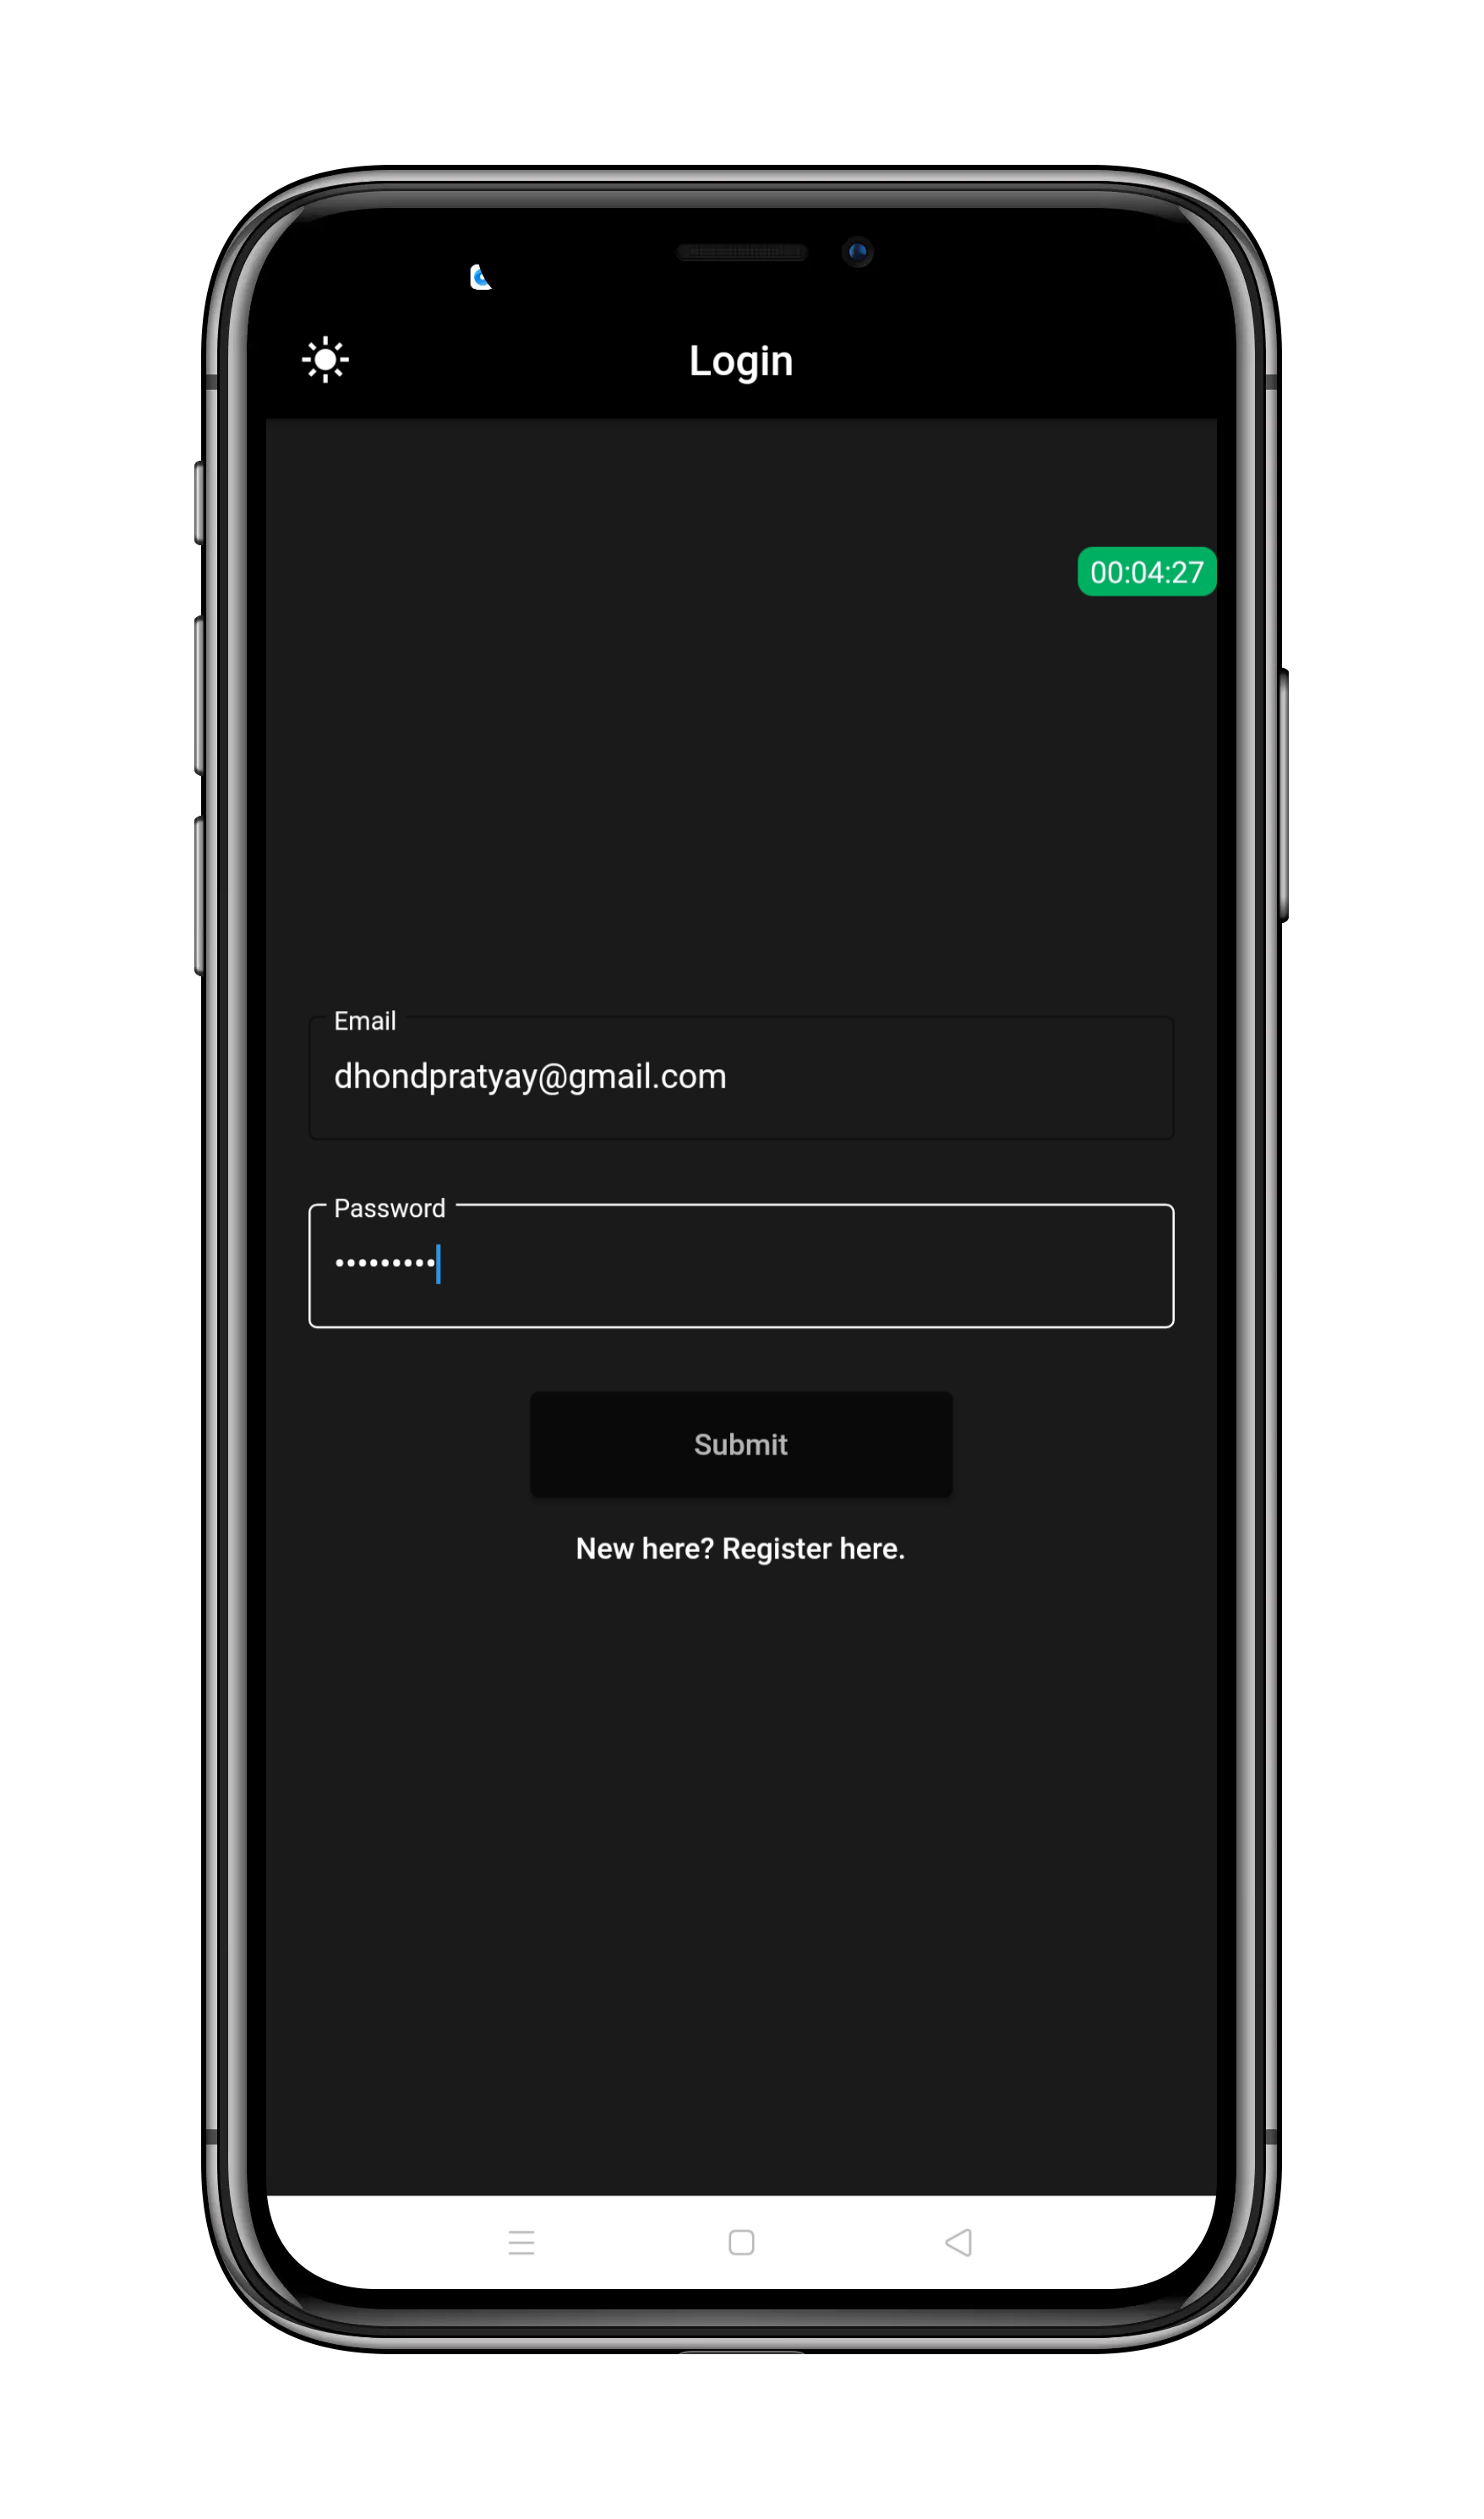
\includegraphics[height=90mm]{Images & Logos/theme/CH_08_Dark_1.png}
  \caption{Login Page}
\end{minipage}%
\begin{minipage}{.5\textwidth}
  \centering
   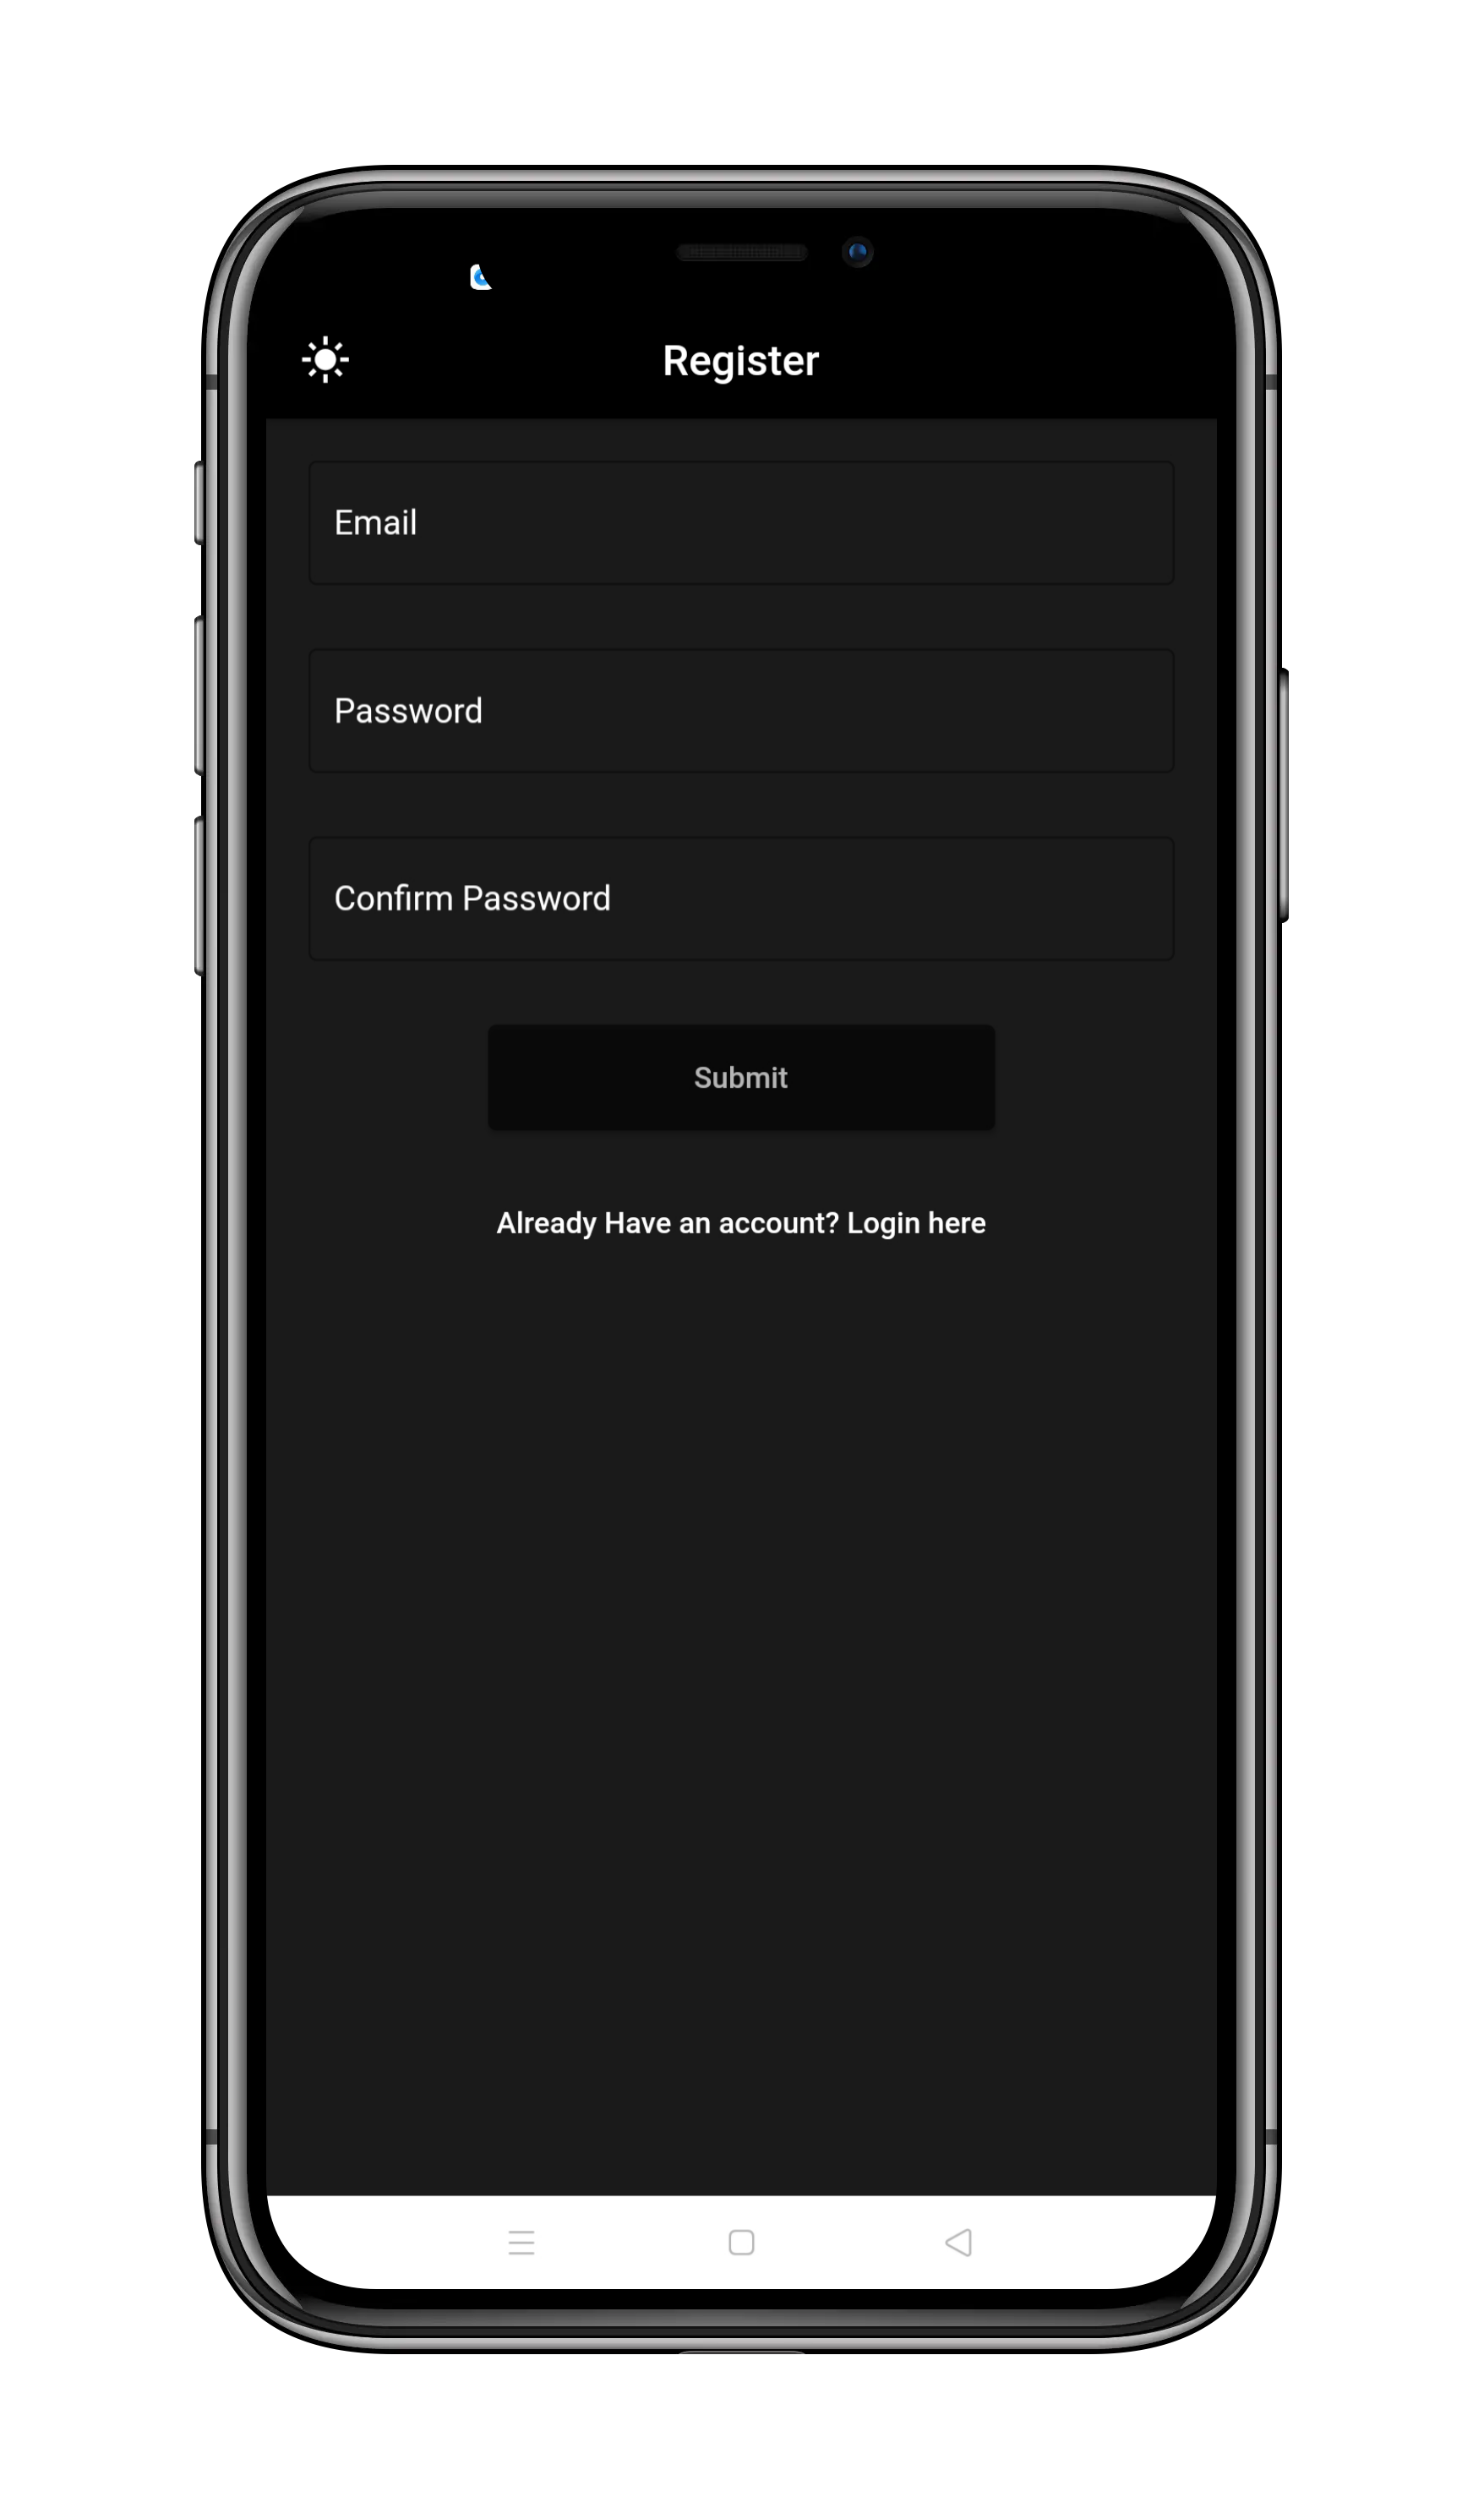
\includegraphics[height=90mm]{Images & Logos/theme/CH_08_Dark_2.png}\\
  \caption{Registration page}
\end{minipage}

\centering
\begin{minipage}{.5\textwidth}
  \centering
   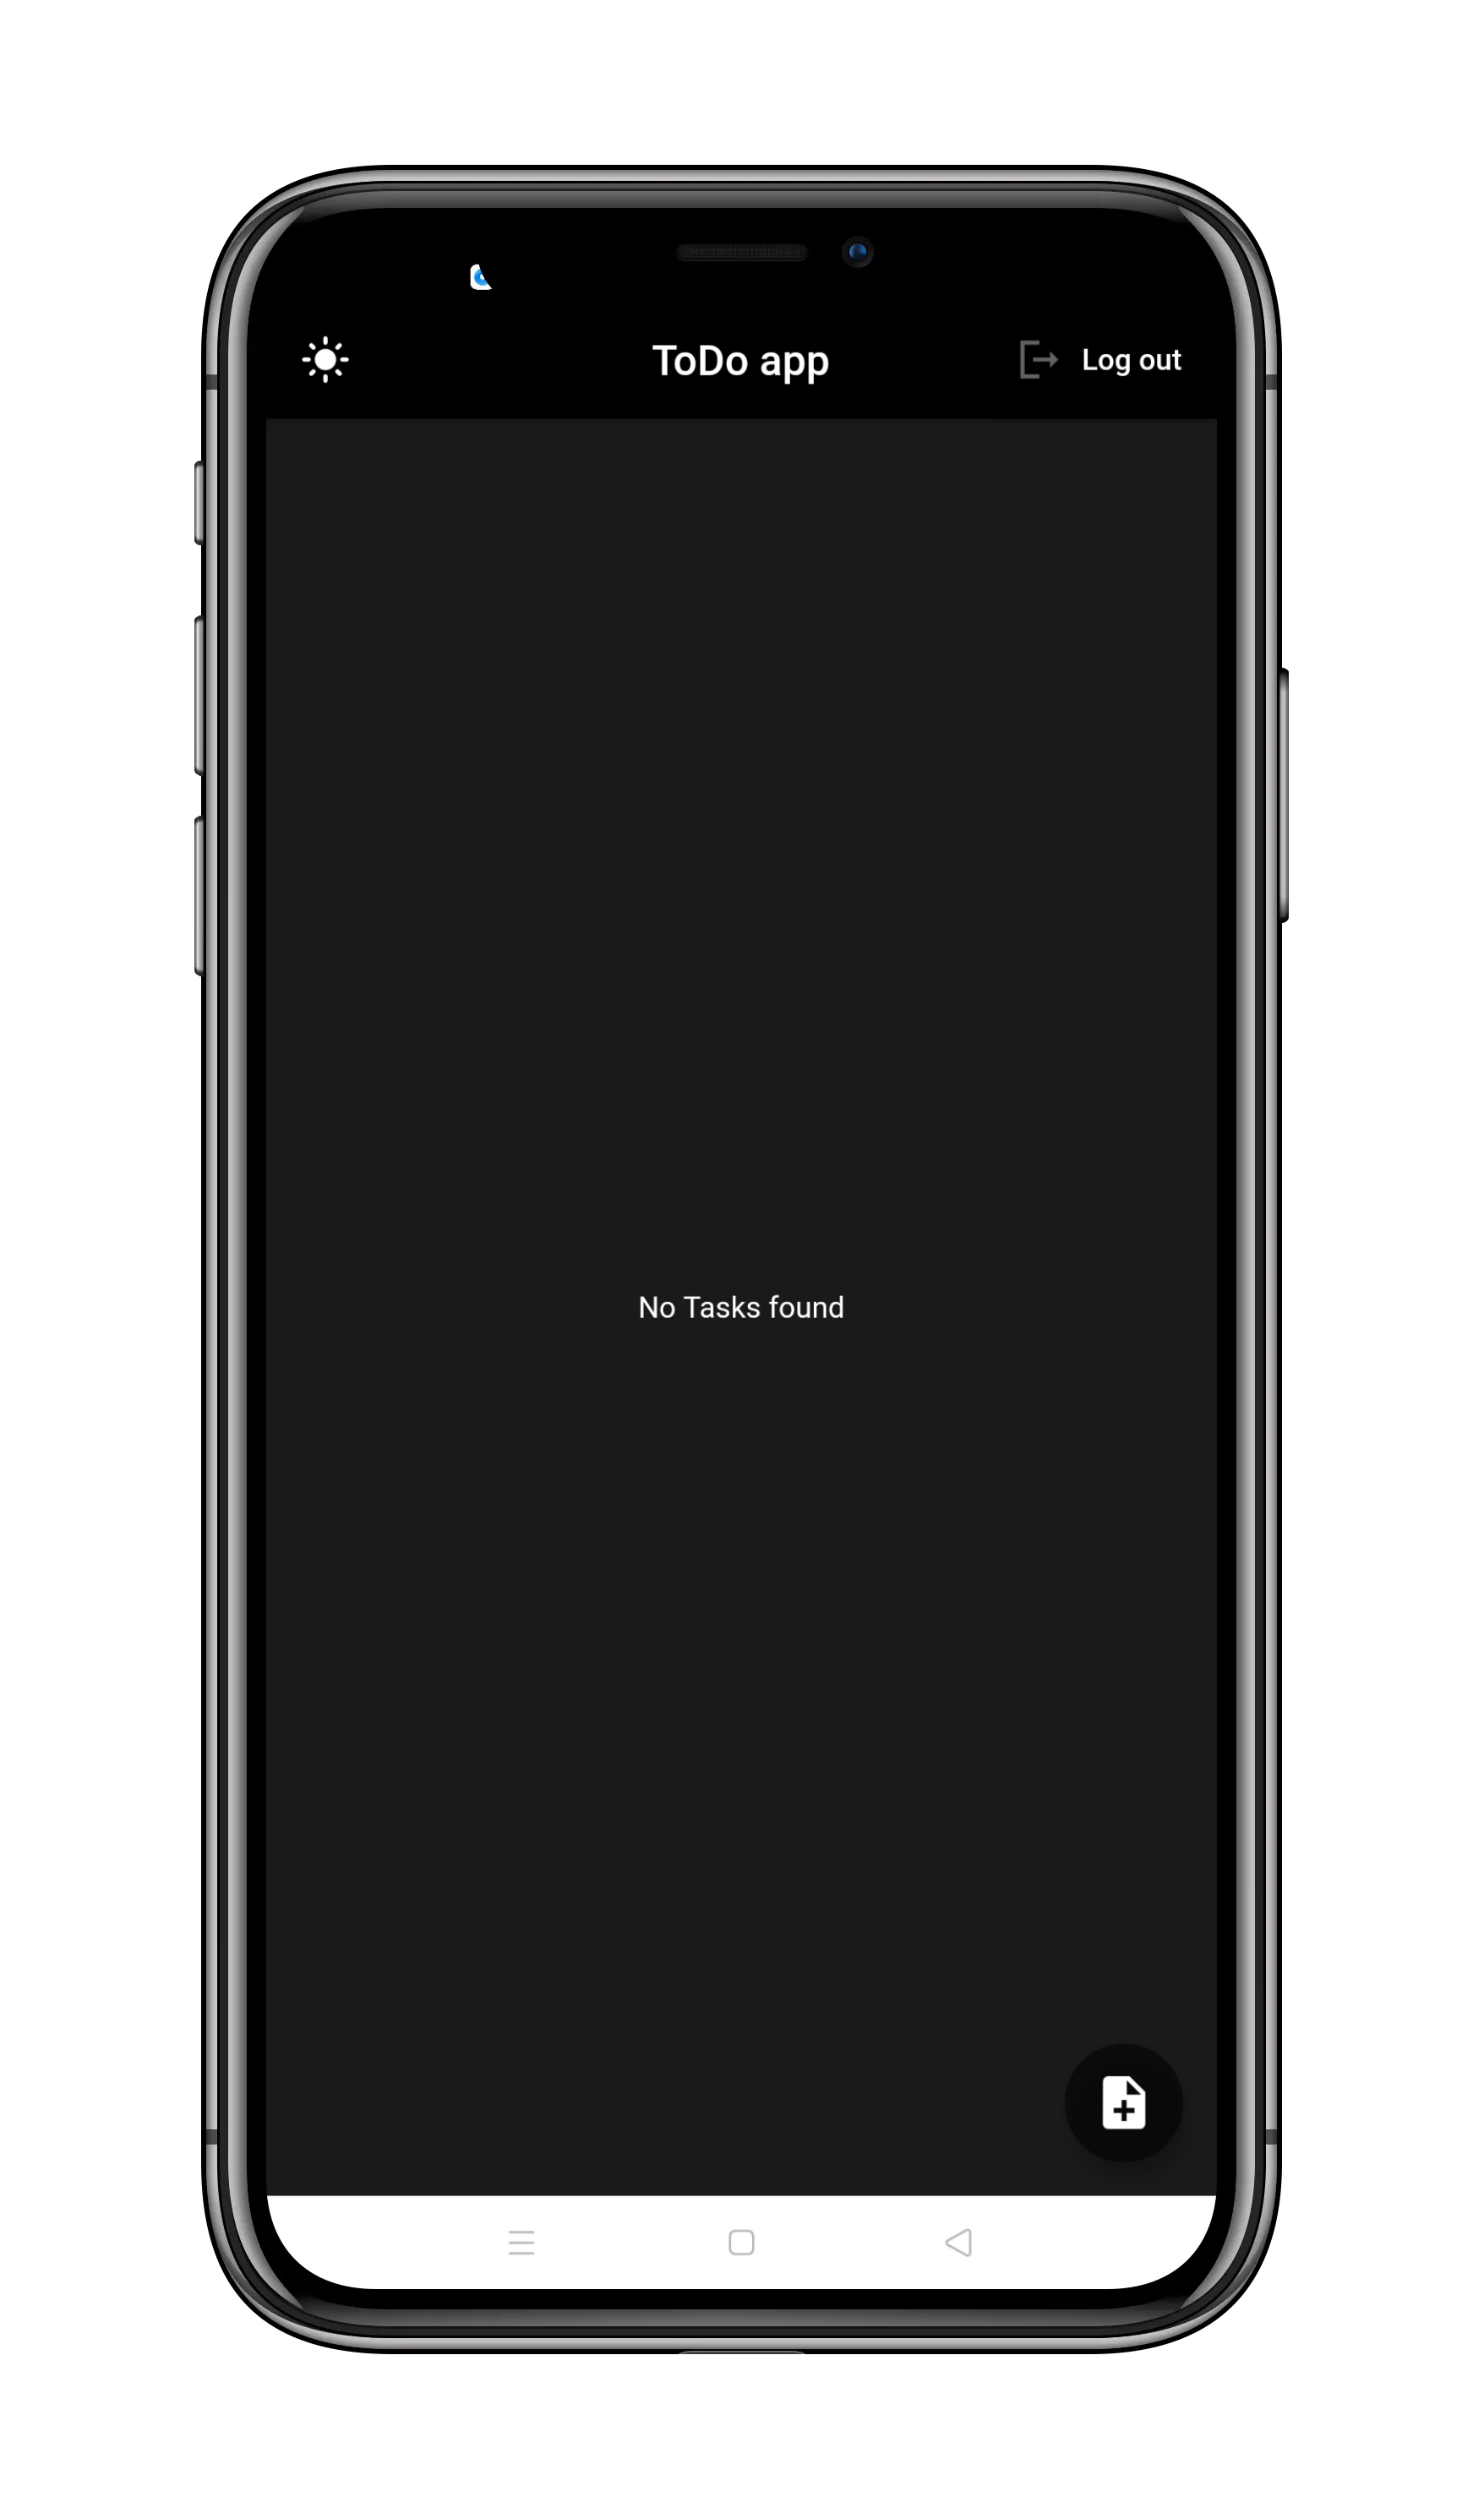
\includegraphics[height=90mm]{Images & Logos/theme/CH_08_Dark_3.png}
  \caption{Home Page}
\end{minipage}%
\begin{minipage}{.5\textwidth}
  \centering
   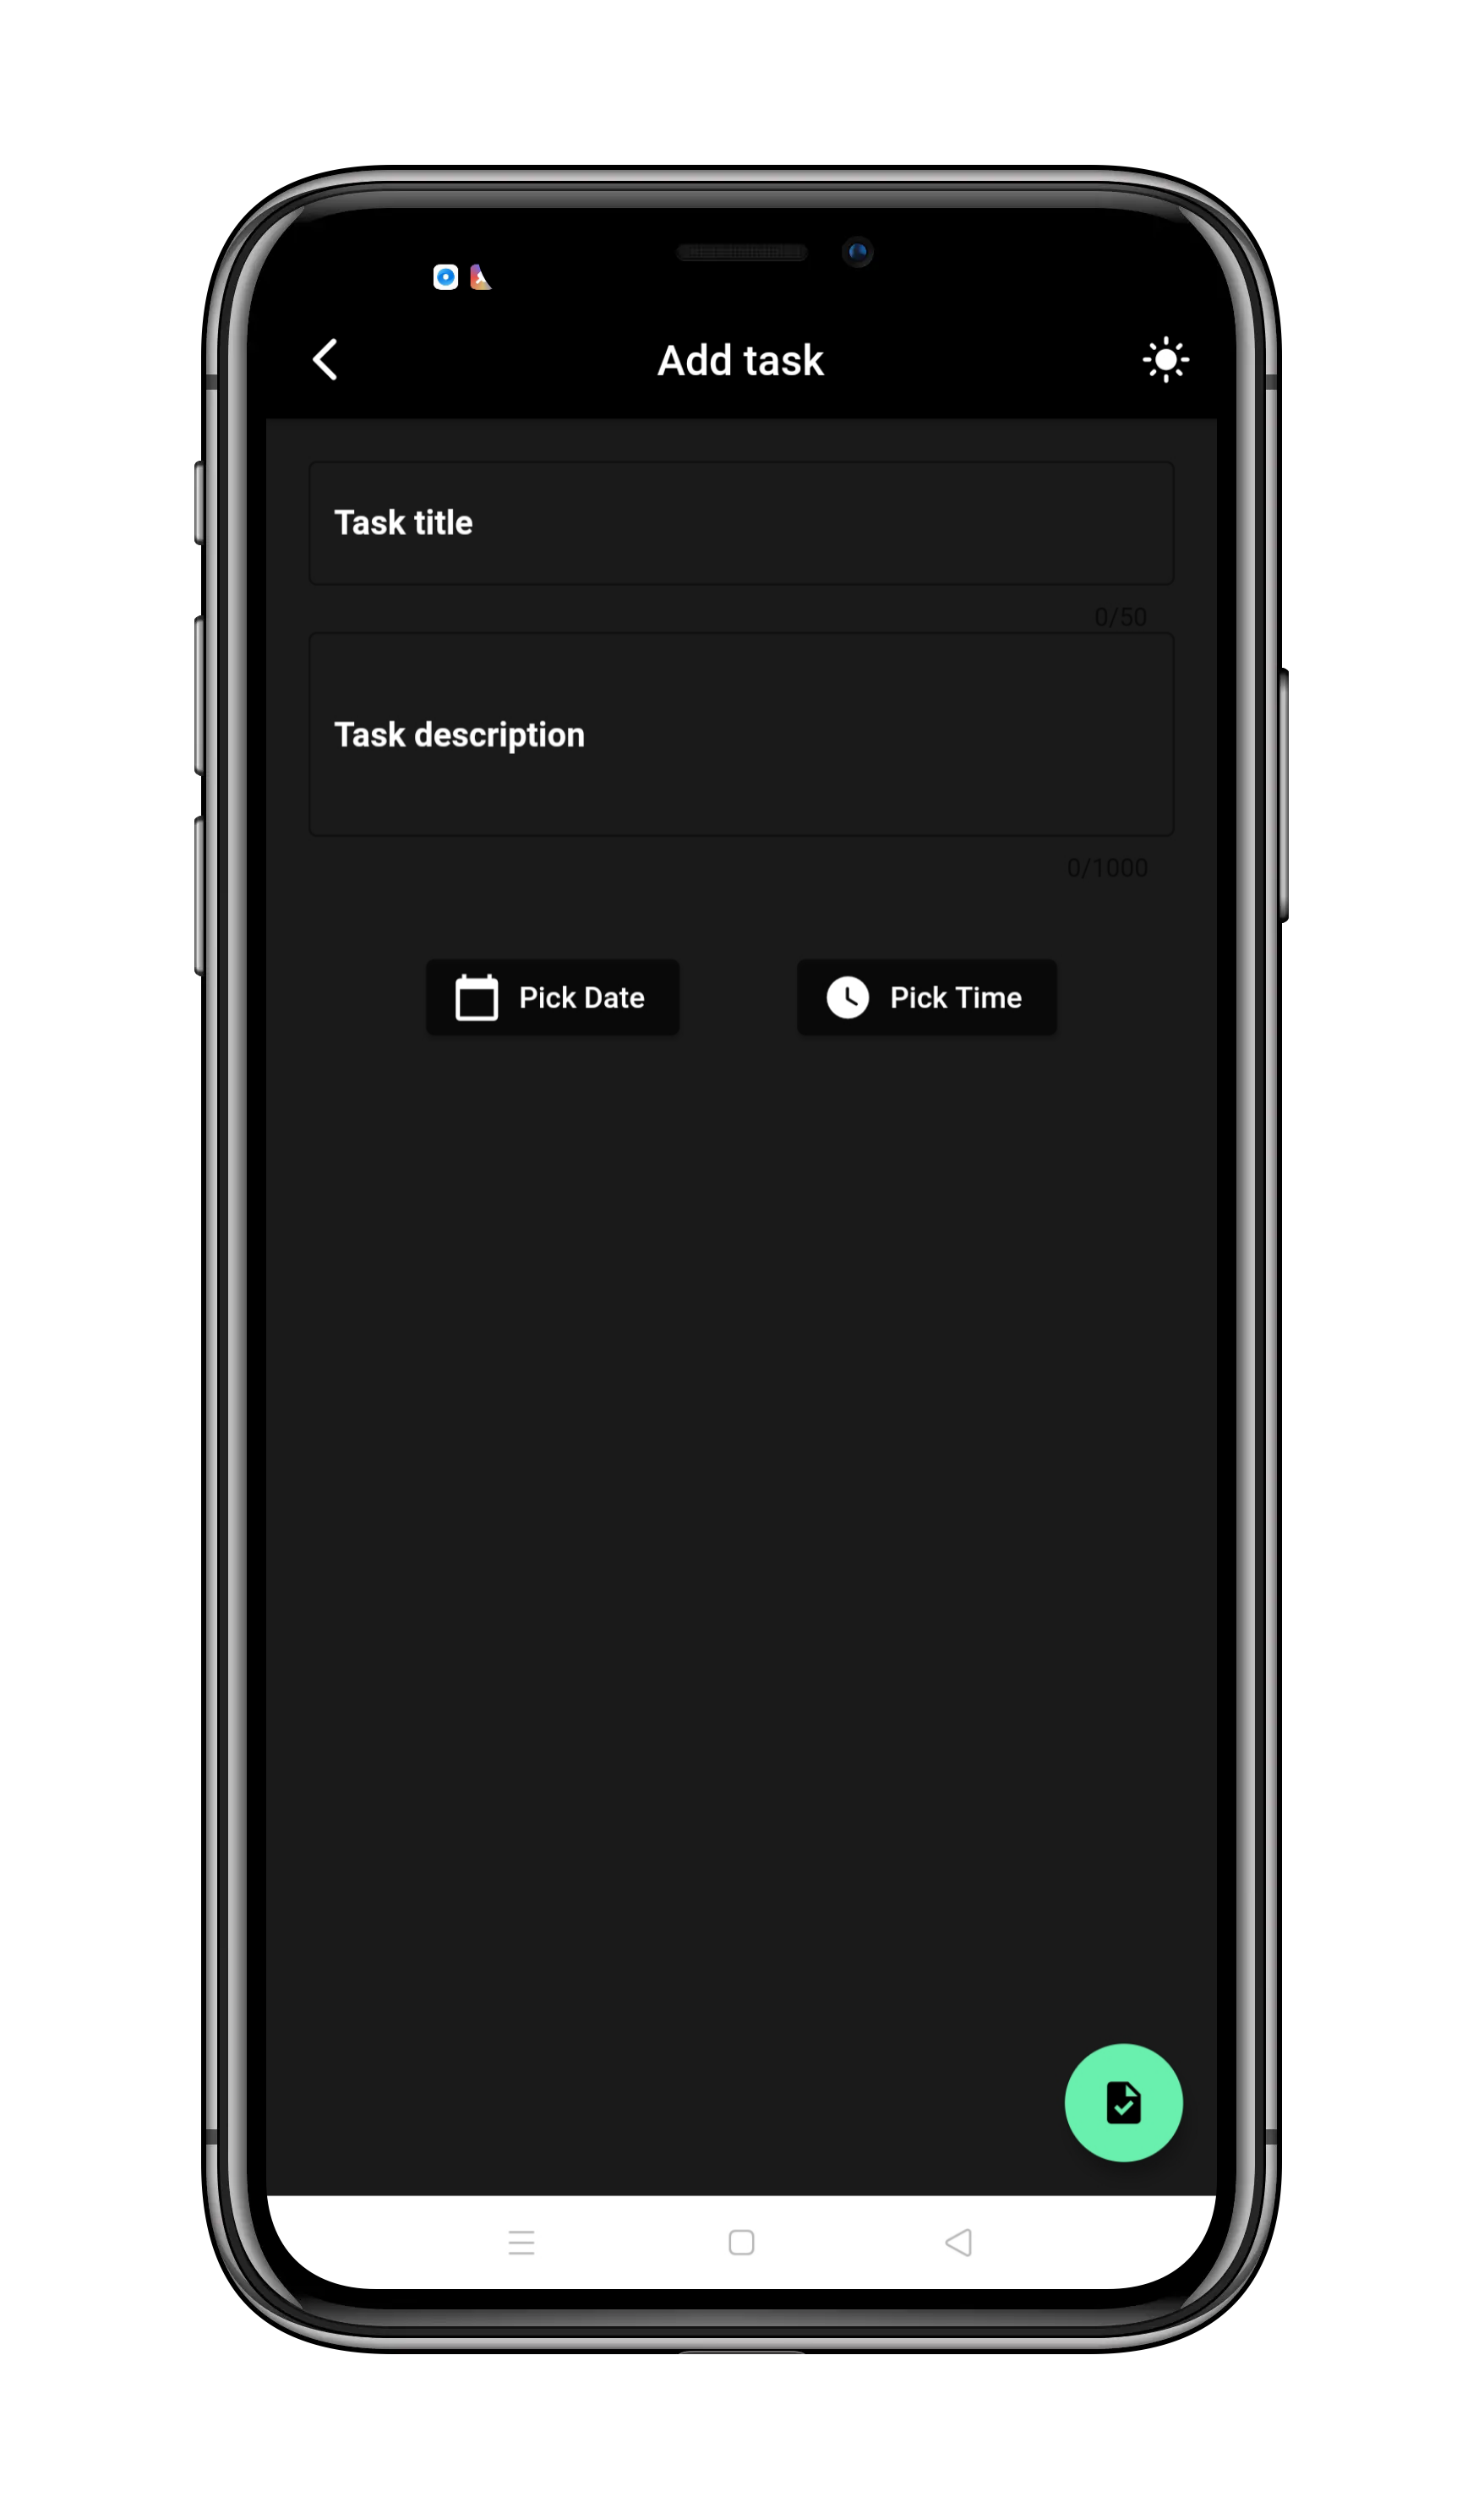
\includegraphics[height=90mm]{Images & Logos/theme/CH_08_Dark_4.png}\\
  \caption{Add Task Page}
\end{minipage}
\newpage
\end{figure}

\begin{figure}[h]
  \begin{center}
   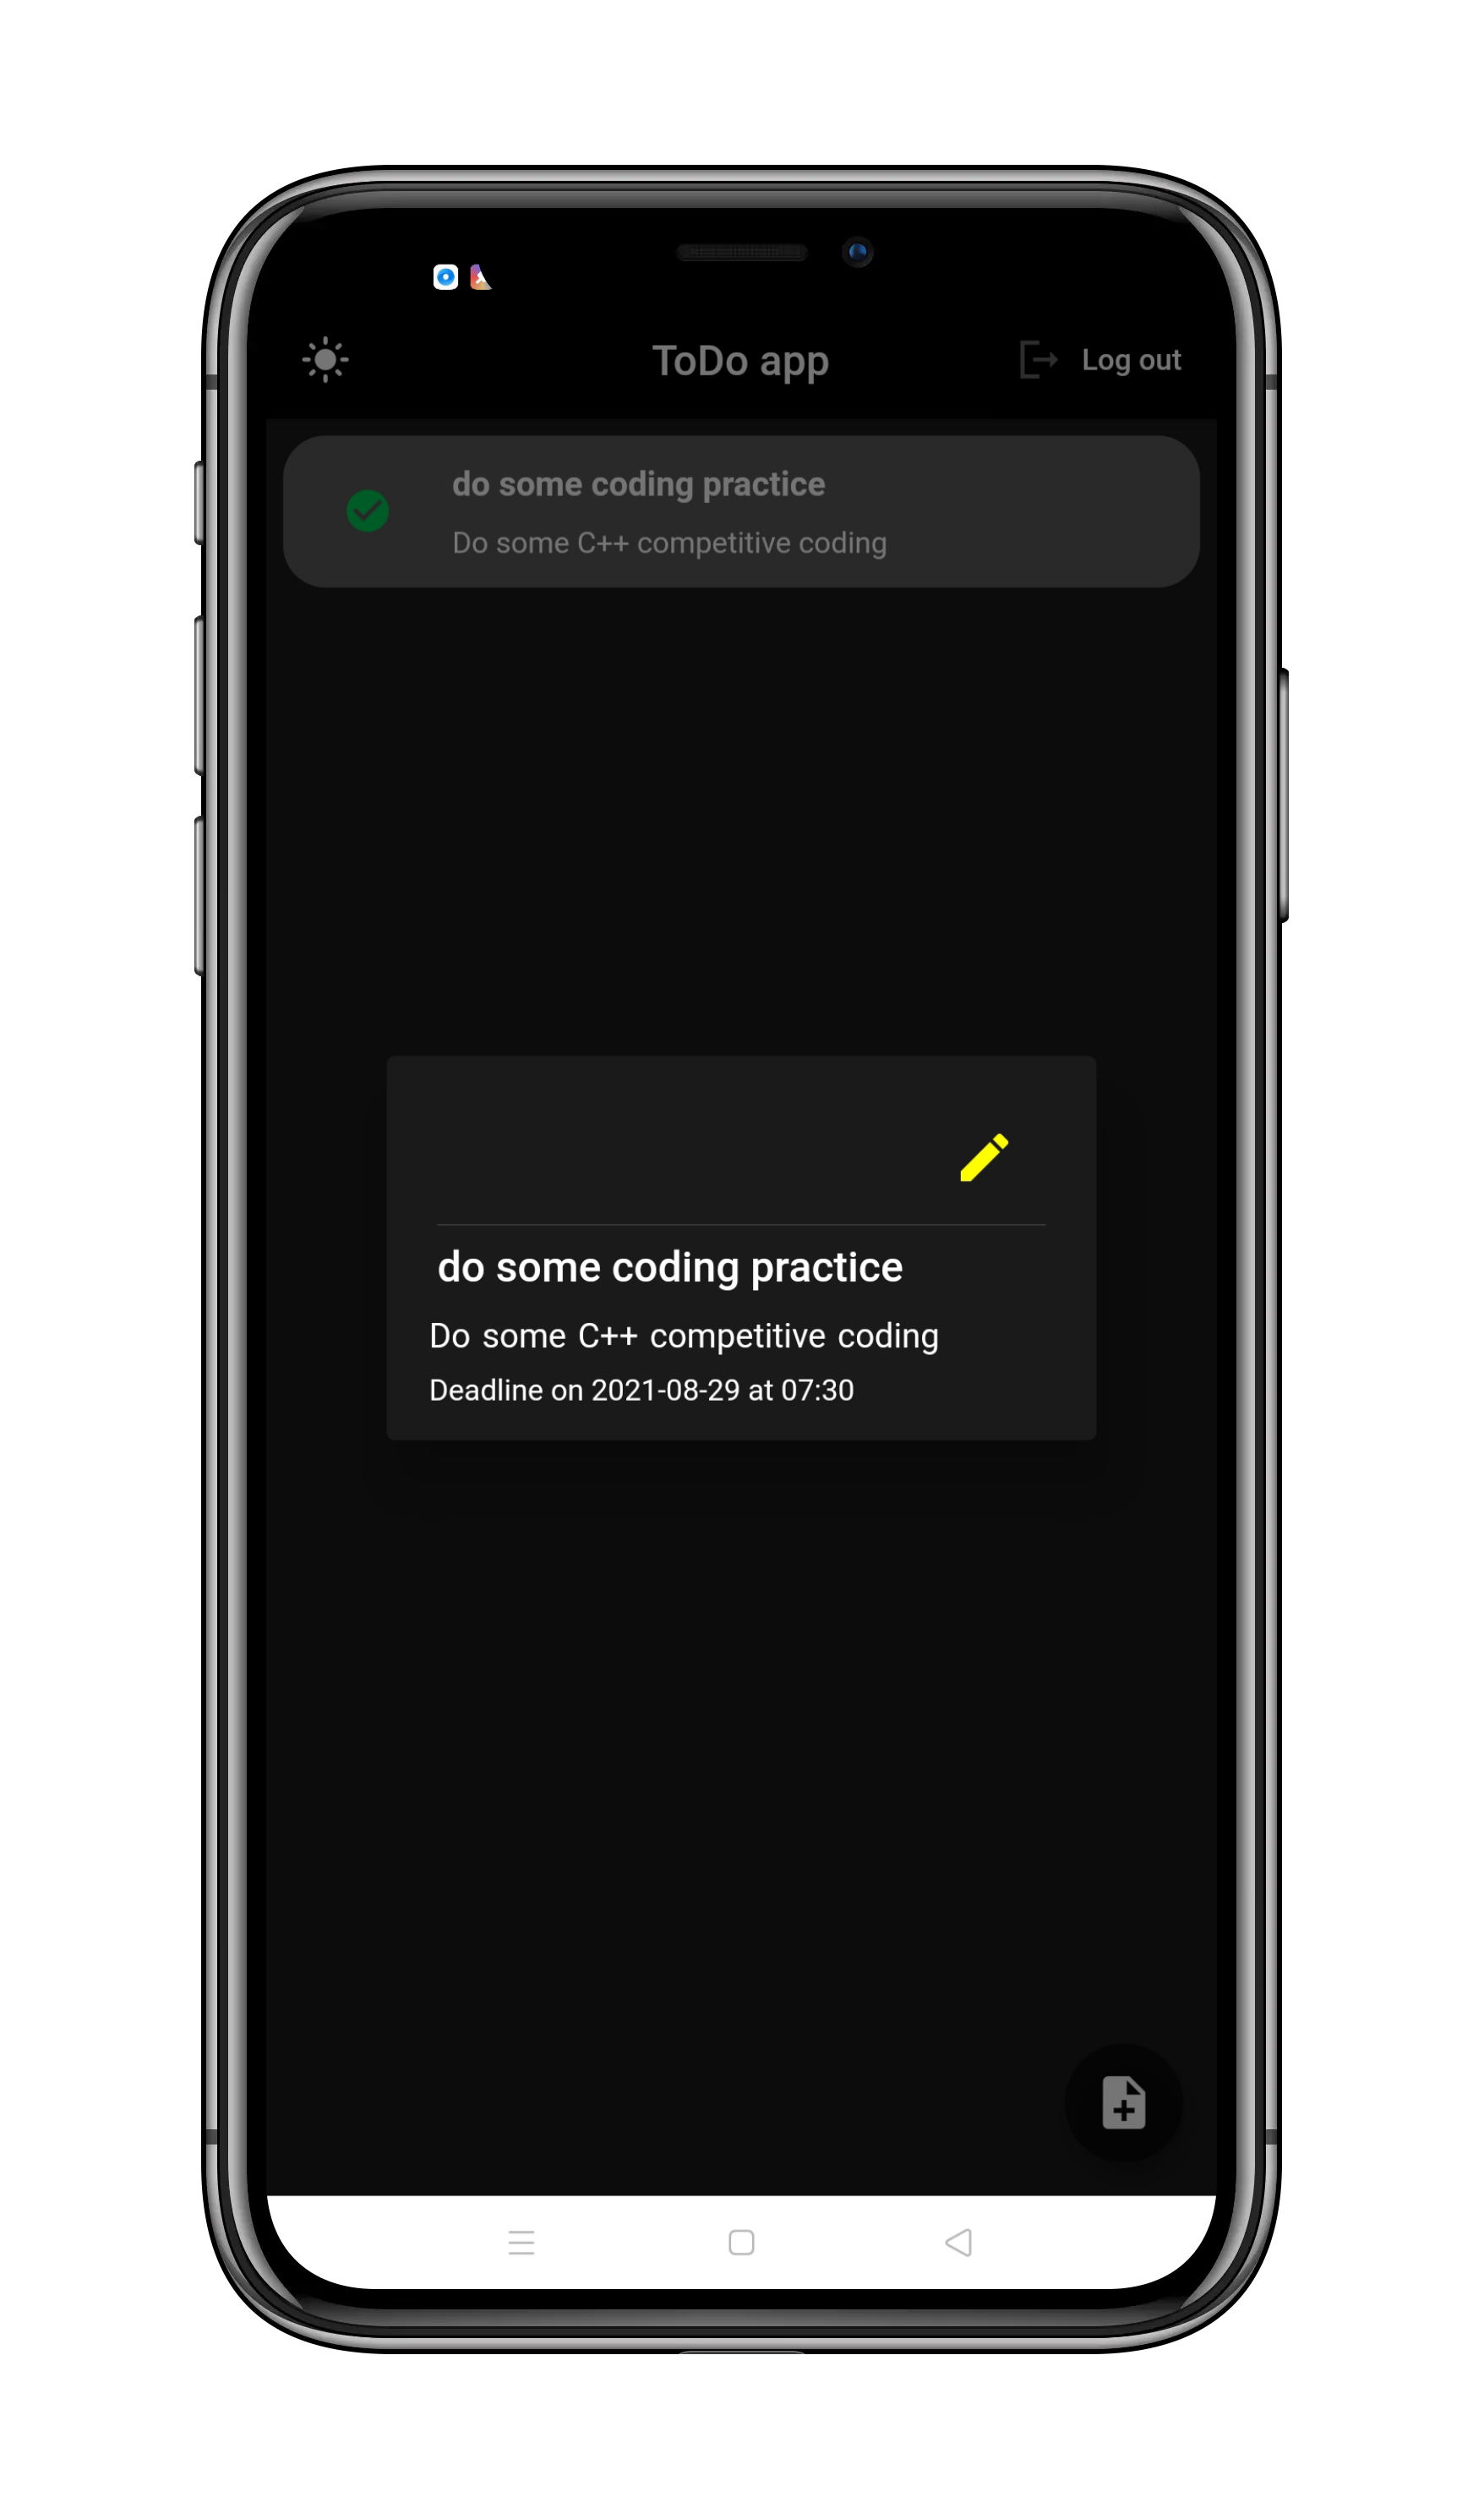
\includegraphics[height=90mm]{Images & Logos/theme/CH_08_Dark_5.png}
%  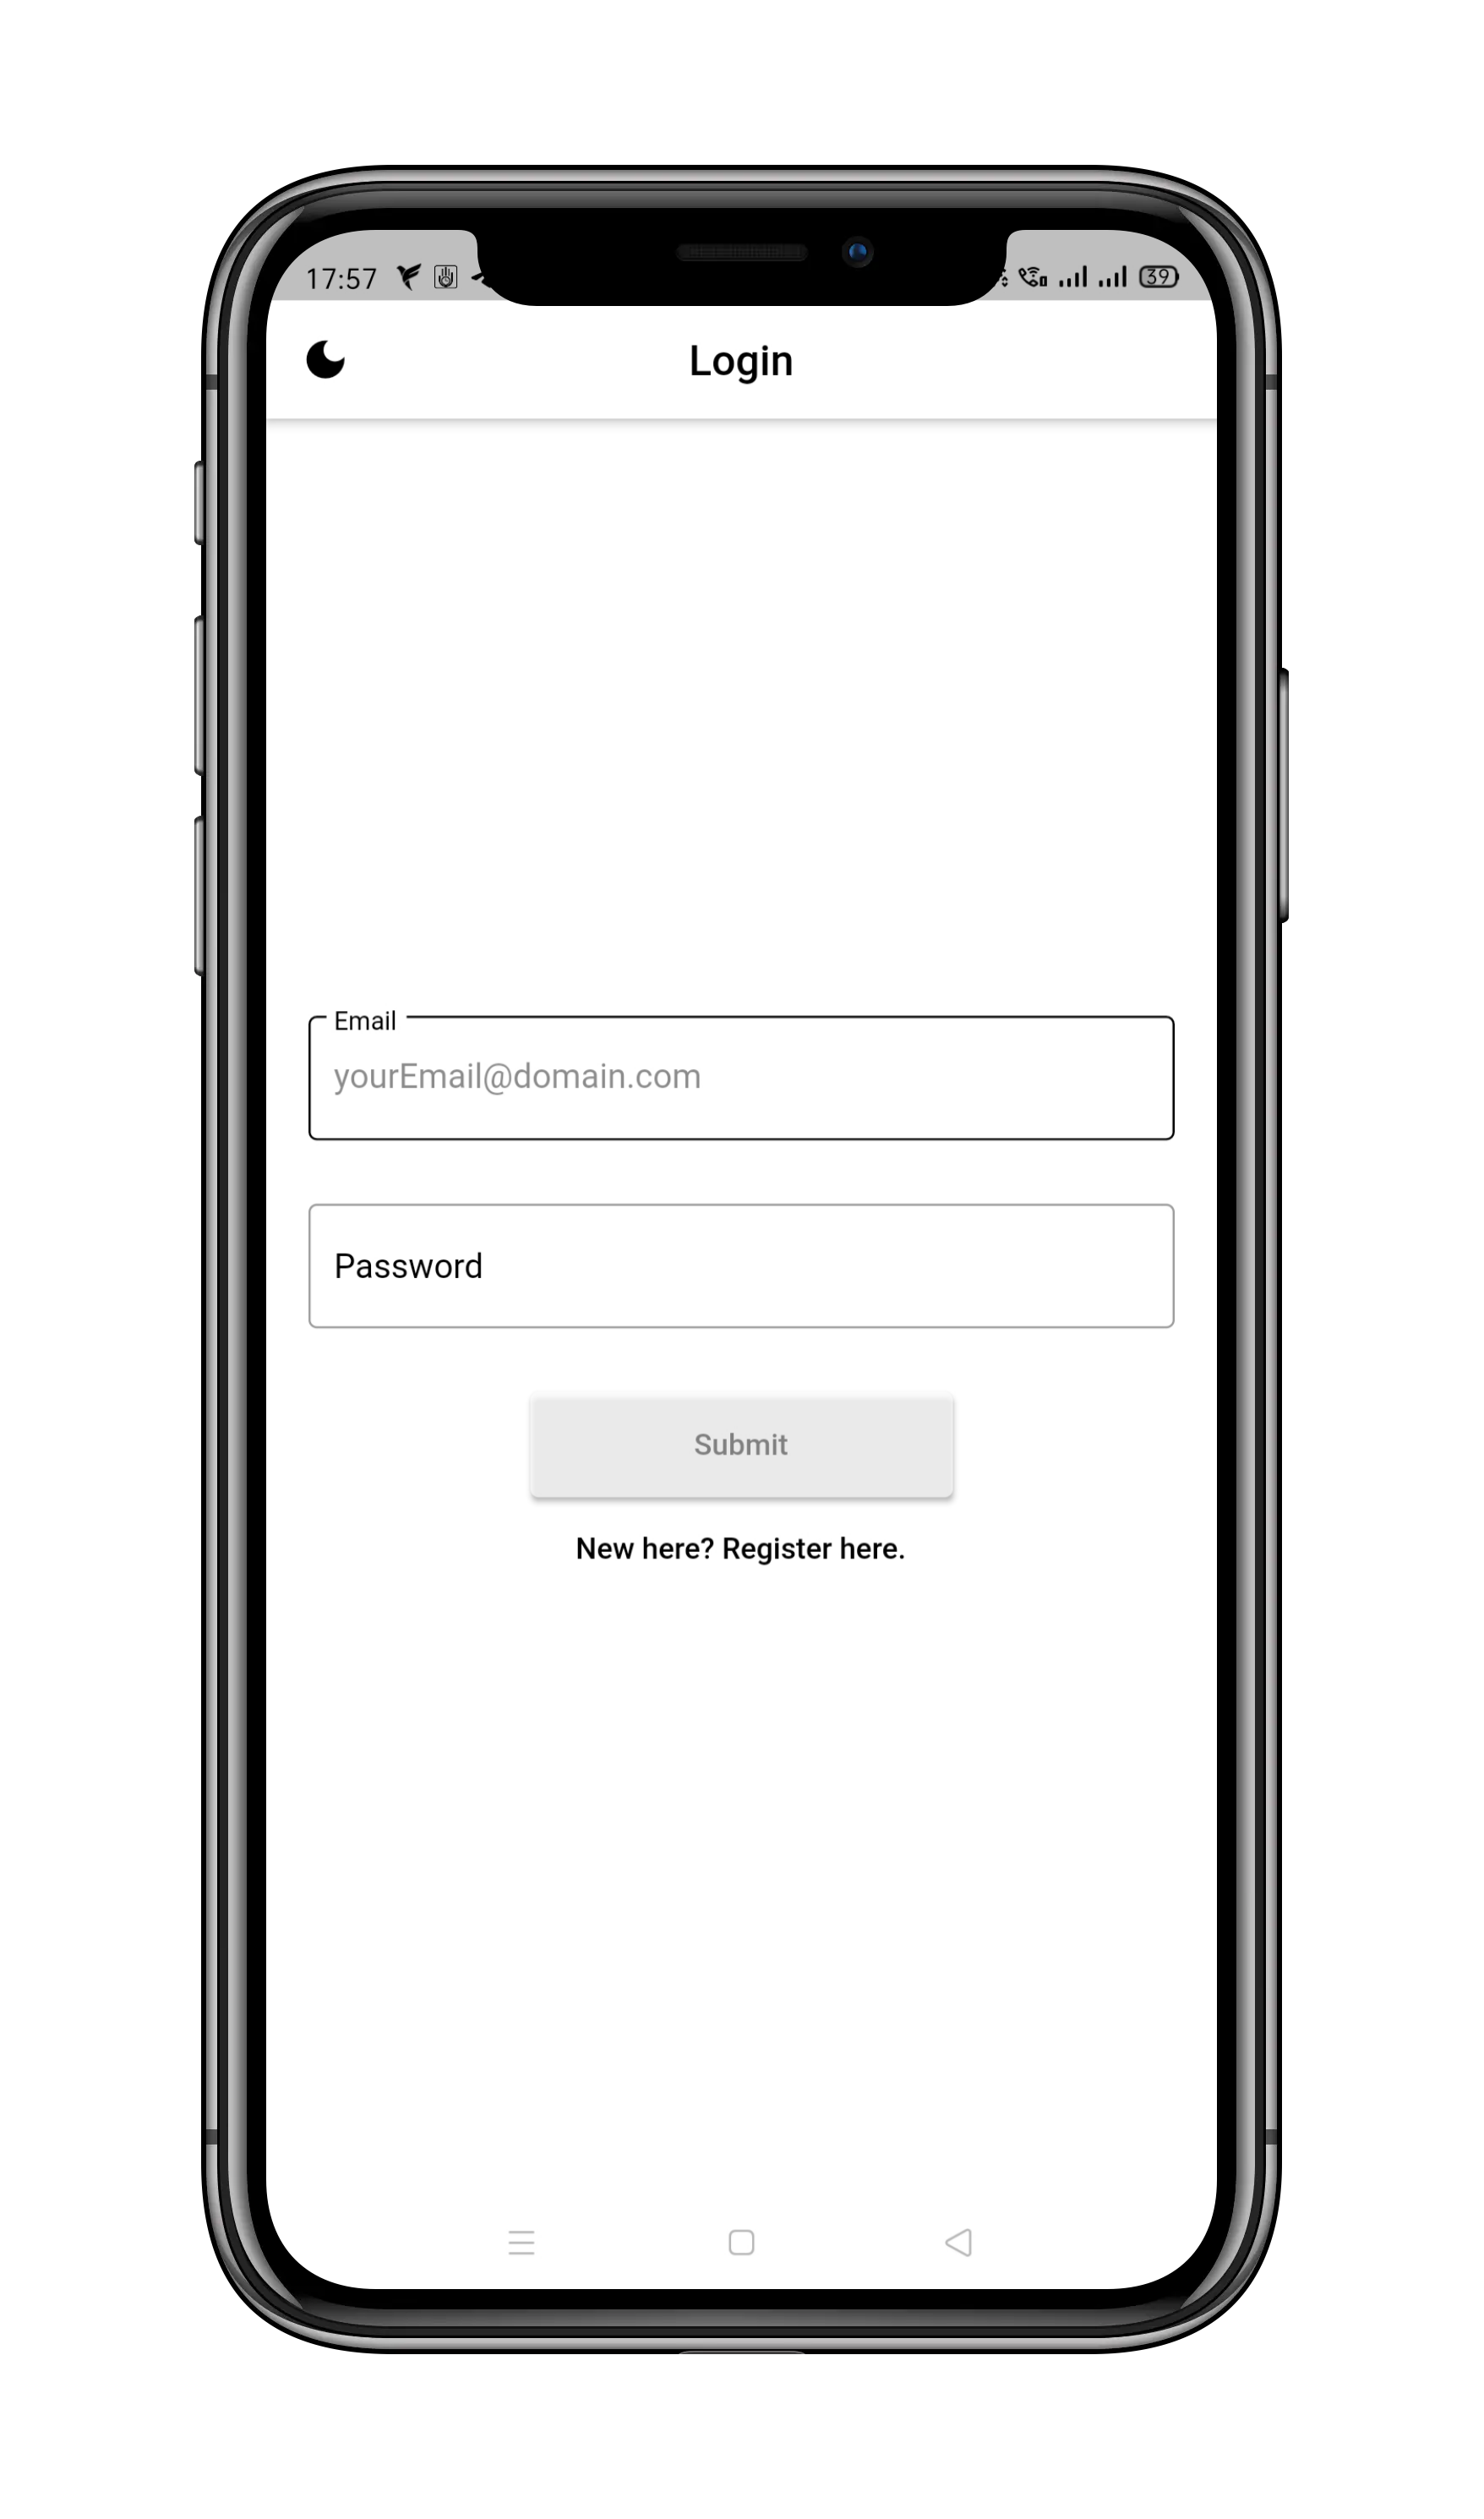
\includegraphics[height=70mm]{Images & Logos/theme/CH_08_Light_1.png}\\
  \end{center}
  \caption{Edit Task Page}
\end{figure}  

.




% \chapter{Future Of Flutter}

Flutter is currently still in beta for windows, Linux and MacOS applications, and is out for pre-release for the web-development. Having Google supporting it is plays a huge role in the success of flutter in the future along with the benefits that flutter offers.\\
	Flutter has a lot of potential and will for sure sustain and make its place in the development environment, as a lot of startups and companies are already switching to Flutter. It can be said that it is soon expected to be capable of overtaking the app development market.

\chapter{Conclusion}
 In the Industrial training in flutter, I learnt about the Flutter framework and the dart programming language, Firestore Firebase database and also about the CRUD operations. I also created an ToDo List app as a project for this internship with two themes and cloud storage so that the tasks can be accessible from any device.\\
 
 The training was an enriching experience for me as I got to know about a lot of industrial practices like 'never to store a password in the database, it should be encrypted' and also 'Not using users gmail id's as an database name but their uid in database' to maintain their anonimity.\\
 
 The main things i have learned through this trainging is time management, working with a team and also Developing cross platform applications using flutter. Working with Flutter has increased my interest in mobile development even more as I was always into android development. Flutter was the spark i needed to enlighten myself and get my interest in development.\\


\nocite{*}
\bibliographystyle{plain}


\chapter{References}
\begin{enumerate}

\item https://flutter.dev/\\
{\em "This is the official website of Flutter."}

\item https://pub.dev/\\
{\em "This is a website where developers can access various open source dependencies and implement them in their project."}

\item https://dart.dev/\\
{\em "This is the official website for Dart programming language."}

\item Practical Flutter - Frank Zammetti\\
{\em "This is a great book for anyone who wants to learn to code using flutter framework and build cross platform apps."}

\item https://www.youtube.com/playlist?list=PLOU2XLYxmsIJ7dsVN4iRuA7BT8XHzGtCr\\
{\em "This is a link to a flutter playlist on youtube made by people working on flutter at google themselves."}

\item https://www.reddit.com/r/FlutterDev/\\
{\em "Flutter forum on reddit contains various doubts, release notes , bugs, bug fixes, etc."}

\item https://discord.com/invite/N7Yshp4\\
{\em "Flutter community on discord is a great place to chat with other flutter developers, post your doubts, solve other people's doubts and to grow better as a developer."}

\end{enumerate}

\end{document}

